% This is samplepaper.tex, a sample chapter demonstrating the
% LLNCS macro package for Springer Computer Science proceedings;
% Version 2.20 of 2017/10/04
%
\documentclass[runningheads]{llncs}

\usepackage{paralist}
\usepackage{graphicx}
\usepackage{amsmath}
\usepackage{amssymb}
\bibliographystyle{splncs04}
% Used for displaying a sample figure. If possible, figure files should
% be included in EPS format.
%
% If you use the hyperref package, please uncomment the following line
% to display URLs in blue roman font according to Springer's eBook style:
% \renewcommand\UrlFont{\color{blue}\rmfamily}

\begin{document}
%
\title{Causal Dynamic Time Lag: Predicting What \& When}
%
%\titlerunning{Abbreviated paper title}
% If the paper title is too long for the running head, you can set
% an abbreviated paper title here
%
\author{Mandar Chandorkar\inst{1,2} \and
Cyril Furtlehner\inst{2} \and
Enrico Camporeale\inst{1} \and 
Michele Sebag\inst{2}
}
%
\authorrunning{Chandorkar et al.}
% First names are abbreviated in the running head.
% If there are more than two authors, 'et al.' is used.
%
\institute{Centrum Wiskunde en Informatica, Amsterdam 1098XG, Netherlands \and
Laboratoire de Recherche en Informatique,
Bât 660 Université Paris-Sud 11,
91405 Orsay Cedex France}
%
\maketitle              % typeset the header of the contribution
%
\begin{abstract}
  We formalize the joint regression task of predicting the magnitude of signals as well as the 
  time delay with respect to their driving phenomena. We call the problem 
  \emph{causal dynamic time lag} (CDT), to take note of the non-stationary time delay between the 
  occurrence of causes/drivers and the observation of effects in physical and man-made systems. 
  We propose a solution to the CDT problem and a methodology to benchmark and evaluate 
  causal time lag estimation algorithms.
\end{abstract}

\section{Introduction}
Exploiting causal relationship between time series is a problem of practical importance 
with many domains of application. Of similar importance is causal relationship between processes. 
Although rigorous understanding and identification of causal links between arbitrary quantities 
is an elusive question, for certain situations it is well known that some causal relationship 
must exist. 

Some of the seminal work relating to causality in time series data is found in \cite{Granger}, 
which introduced the concept of \emph{Granger Causality}. \emph{Granger causality} focused on the 
problem of predictive causality instead of the philosophical or \emph{true causality}. Although 
originally formulated for linear causal relationships with no latent variables, it has since been 
extended for various situations (see \cite{doi:10.1002/9781119945710.ch22} for a review).

In temporal phenomena, it is also the case that causal effects of events are not immediately observed, 
but after a certain time interval which can be dynamic. One prominent example of such behavior is the
 Sun-Earth system and its associated problem of space weather forecasting.

The Sun, a perennial source of charged energetic particles ejects them into the surrounding space. 
This particle cloud or \emph{solar wind} reaches the Earth's vicinity and interacts with its 
magnetic field in complex ways, giving rise to geomagnetic phenomena. High speed solar wind can 
potentially cause damage to under sea pipelines, satellites, and other telecommunication 
infrastructure. A key prediction task is to forecast the speed of the \emph{solar wind} in 
the vicinity of the Earth from solar image data 
(\cite{doi:10.1002/jgra.50429}, \cite{doi:10.1029/2009SW000542}).

The \emph{solar wind} forecasting problem can be broken down into two stages. First, the extraction of 
features from solar images and second, the prediction of time lagged solar wind speed near the Earth. 
In this work we present progress made on the second part of this problem.
 
To our knowledge, the problem of regression with hidden non-constant time delay, as formulated later in 
section \ref{sec:formulation} has not been addressed in the machine learning literature. 

Similar type of problems have actually been encountered in the context of financial time series 
prediction in \cite{ZHOU2006195} for instance. Their approach is a form a dynamical time warping (DTW) 
which appeared originally in the context of speech recognition~\cite{SakoeShiba1978}. 
\cite{SignalDiffusion} build on the DTW paradigm and take a Bayesian approach to the temporal alignment 
problem between time series. However they limit themselves to linear relationships between 
the input and output time series, assuming in addition slow varying time lags.

The DTW algorithm and its variants are now widely used in time series analysis, but they always assume 
a predefined cost matrix for the temporal alignment between two time series and they assume the 
causes $x(t)$ and effects $y(t)$ are of same dimensionality and structure. 

Our work has the following novel characteristics as compared to the DTW paradigm.

\begin{enumerate}
    \item Causes and effects are of different dimensionality. The output time series $y(t)$ is scalar, 
          but its driver $x(t)$ is potentially high dimensional, e.g. vectors, images etc.
    \item We do not make assumptions as made in \cite{ZHOU2006195} and other 
          \emph{dynamic time warping} related works about the time lag function. 
          In our case the time lag can be potentially non smooth.
    \item The relationship between $x(t)$ and $y(t)$ can be potentially non-linear. 
\end{enumerate}


\section{Problem Formulation}\label{sec:formulation}

\subsection{CDT: Formulation}

\emph{Causal Dynamic Time Lag} (CDT) is essentially a regression problem with two tasks. 
Given two time series, the causes $x(t)$ and the observed effects $y(t)$, the regression model 
must learn a mapping $f(.)$ which maps each input pattern $x(t_1)$ to an output $y(t_2)$, and a 
mapping $g(.)$ which maps the time delay between the input and output patterns $t_2 = t_1 + g(x(t_1))$. 
This is formally specified in equations below.

\begin{align}
y(t + \tau(t)) & = f[x(t)]\label{eq:pb1}\\
\tau(t) & = g[x(t)]\label{eq:pb2} 
\end{align}
with
\[
f: \mathcal{X}  \rightarrow \mathbb{R},\qquad\text{and}\qquad
g: \mathcal{X}  \rightarrow \mathbb{R}^{+},
\]
$t \in \mathbb{R}^{+}$ represents the continuous temporal domain. The input signal 
$x(t)\in \mathcal{X}$ is possibly high dimensional and contains the hidden cause to 
the effect $y(t)\in\mathbb{R}$ which is considered as a scalar in this paper. 
$\Delta(t)\in \mathbb{R}^+$ represents the time delay between cause and effect.

It is important to note some caveats about this causal time lag which make the CDT different from 
classical time series regression problems.

In practical applications such as the motivating space weather example, $\Delta(t)$ is not recorded 
explicitly in the data set. This makes model training and evaluation challenging.

One may make certain assumptions on the time warping function $\phi(t) = t + g(x(t))$, in the general 
formulation of the problem presented here: 

\begin{enumerate}
    \item $\phi(.)$ is assumed to be continuous and \emph{bijective}.
    \item Zhou \& Sornette \cite{ZHOU2006195} enforce further assumptions such as 
          $\phi(t_1) \leq \phi(t_2), \forall t_1 \leq t_2$, which are incorporated via constraints. 
          This approach respects the properties associated with the warping function $\phi(.)$ but 
          increase the computational complexity of the resulting optimization problem.
\end{enumerate}

The second assumption can be restrictive for applications in space physics, where fast moving 
solar wind can reach the Earth before slow moving solar wind which departed before it. 

\subsection{CDT: A Probabilistic Perspective}\label{sec:cdtprobform}

It is an interesting exercise to consider casting the CDT problem in a probabilistic framework.
As we shall see below, a probabilistic formualtion will lead us to a possible solution method
for the CDT problem. 

\begin{align} \label{eq:cdtprob}
      &y(t) = \int_{0}^{\infty}{f[x(t - \tau)] \rho(t, \tau, x(t - \tau))}d \tau \\
      & \nonumber \rho(t, \tau, x(t - \tau))  = \delta(\tau - g[x(t - \tau)])
\end{align}

In \ref{eq:cdtprob}, we express the output time series $y(t)$ as a convolution between
the output mapping $f(.)$ from section \ref{sec:formulation} and a \emph{causal probability}
distribution $\rho(t, \tau, x(t - \tau))$. 

The \emph{causal probability distribution} $\rho(t, \tau, x(t - \tau))$ expresses the probability 
that $y(t)$ is caused by $x(t - \tau)$. The quantity $\tau$ is thus the \emph{causal time lag}. 
As cause is assumed to preceed effect, the time lag is assumed to be strictly positive ($\tau \geq 0$). 
The support of the \emph{causal probability} distribution is thus $\mathbb{R}^+$.

In order to recover the relationships in equations \ref{eq:pb1} and \ref{eq:pb2}, we 
set the \emph{causal probability} distribution to the dirac delta function centered
around $g[x(t - \tau)]$.

\subsection{Likelihood formulation in the discrete case}
Suppose we discretize time in units of $\delta t$, such that for a given event $x^{(m)}$ at time  $t = m\ \delta t$, the possible time lag $\tau^{(m)}$ is within a window
$[\tau_{min},\tau_{max}]$. This interval is as well discretized into $n = (\tau_{max}-\tau_{min})/\delta t $ intervals so that the effect if any of this event has to be found in the vector of size $n$ of possible effects denoted ${\bf y}^{(m)} = \{y_1^{(m)},\ldots,y_n^{(m)}\}$.
Our probabilistic formulation is given by the following conditional probability distribution:
\begin{align*}
P\bigl[{\bf y}^{m} = {\bf y}\vert x^{(m)}=x\bigr] &= \\[0.2cm] \sum_{\{\tau_i\in\{0,1\}\}}
& \tilde p\bigl(\tau_1,\ldots,\tau_n\vert x)
\frac{1}{(2\pi)^{n/2}\prod_i\sigma(\tau_i)}
\exp\Bigl(-\frac{1}{2}\sum_{i=1}^n\frac{\bigl(y_i-\hat y_i(x)\bigr)^2}{\sigma(\tau_i)^2}\Bigr),
\end{align*}
with 
\[
\sigma(\tau)^2 = \frac{\sigma^2}{1+\alpha \tau},
\]
with $\sigma^2$ a default variance and $\alpha\ge 0$ a non-negative real parameter and $\hat y(x)$ a vector of mean effects corresponding to a given cause $x$. 
The meaning of this is the following: for a given cause $x$ the effect
$y_i$ at horizon $i$ has a normal distribution centered on $\hat y_i(x)$ with  variance $\sigma^2(\tau_i)$ independent of $x$ as a simplifying assumption. $\{\tau_1,\ldots,\tau_n\}$ is a set of binary latent variables encoding the stochastic causal time lag, by telling whether $x$ causes $y_i$ ($\tau_i=1$) or not ($\tau_i=0$). Since we expect approximately a one to one correspondence between causes $x_t$ and effect $y_{t+\tau(t)}$ we impose on the joint probability $\tilde p(\tau_1,\ldots,\tau_n\vert x)$ the constraint
\begin{equation}\label{eq:cs1}
\mathbb E\Bigl(\sum_{i=1}^n \tau_i\vert x \Bigr) = 1,
\end{equation}
which means that $x$ causes one single effect in average among the $n$ possible ones. The fact that $x$ can influence $y_i$ through the bias $\hat y_i(x)$ even when $\tau_i=0$ reflects an indirect influence due to a finite auto-correlation time of $y_t$. But this comes with a higher variance, 
since $\sigma(0)^2\ge \sigma(1)^2$, controlled by the parameter $\alpha$.
A large value of $\alpha$ should correspond to a small auto-correlation time. Remains then to specify 
$p(\tau_1,\ldots,\tau_n\vert x)$. In this paper we chose the simplest possibility, namely a product of independent variables:
\[
\tilde p(\tau_1,\ldots,\tau_n\vert x)= \prod_{i=1}^n \tilde p_i(\tau_i\vert x),
\]
with the constraint (\ref{eq:cs1}) reading
\[
\sum_{i=1}^n \tilde p_i(\tau_i=1\vert x) = 1.
\]
We are now in position to justify the loss function which will be used later on to train our model, as arising from a large deviation functional of the likelihood. Indeed assume that the number of learning samples tends to infinity, and so that in a small volume $dv = dxd\bf y$ around a given  joint configuration $(x,\bf y)$, the number of data $N_{x,\bf y}$ becomes large. Restricting the likelihood to this subset of the data yields the following:
\[
{\cal L}_{x,{\bf y}} = \prod_{m=1}^{N_{x,{\bf y}}} \sum_{\{\tau^{(m)}\}}\prod_{i=1}^n 
\frac{\tilde p_i(\tau_i^{(m)}\vert x)}{\sqrt{2\pi}\ \sigma(\tau_i^{(m)})}
\exp\Bigl(-\frac{1}{2}\sum_{i=1}^n\frac{\bigl(y_i-\hat y_i(x)\bigr)^2}{\sigma(\tau_i^{(m)})^2}\Bigr).
\]
Upon introducing the (discrete) counting measures:
\[
\hat p_i = \frac{1}{N_{x,{\bf y}}}\sum_{m=1}^{N_{x,{\bf y}}} \tau_i^{(m)} 
\]
the sum over the $\tau_i^{(m)}$ is replaced by a sum over these new variables, with the summand obeying a large deviation principle (see e.g.~\cite{Touchette})
\[
{\cal L}_{x,{\bf y}} \asymp \sum_{\hat {\bf p}} 
\exp\Bigl(-N_{x,{\bf y}} {\cal F}_{x,{\bf y}}\bigl[\hat {\bf p}\bigr]\Bigr)
\]
where the rate function simply reads from Sanov's theorem
\[
{\cal F}_{x,{\bf y}}\bigl[\{\hat p\}\bigr] = n\log(\sigma)+
\frac{1}{2}\sum_{i=1}^n\Bigl[\bigl(y_i-\hat y_i(x)\bigr)^2\frac{1+\alpha\hat p_i}{\sigma^2}
+\hat p_i\log(1+\alpha)+\hat p_i\log\frac{\hat p_i}{\tilde p_i}\Bigr].
\]
Taking the saddle point yields the following:
\[
\hat p_i(x,{\bf y}) = \frac{1}{\sqrt{1+\alpha}}\tilde p_i(x)\exp\Bigl(-\frac{\alpha}{2\sigma^2}\bigl(y_i-\hat y_i(x)\bigr)^2\Bigr).
\]
In summary we have two coupled regression problems $\hat {\bf y}(x)$
and $\hat {\bf p}(x)$ to solve, with loss function ${\cal L}\bigl[\hat {\bf y},\hat {\bf p}\bigr]$ identified to the empirical mean over the dataset of the rate function ${\cal F}_{x,{\bf y}}\bigl[\hat {\bf p}\bigr]$.







\section{Proposed Solution}\label{sec:model}

From section \ref{sec:cdtprobform}, we can express the probabilistic CDT regression 
problem as the learning of two tasks.

\begin{enumerate}
    \item Generate accurate predictions for $y(t + \tau)$
    \item Learn the \emph{causal probability} distribution $\rho(t + \tau, \tau, x(t))$.
\end{enumerate}

The model therefore must consist of two estimators:
\begin{inparaenum}[1.]
      \item Output $\hat{y}(t + \tau)$
      \item Causal probability $\hat{p}(t + \tau, x(t))$.
\end{inparaenum} 
We have access to measurements of the output time series $y(t)$, but that is 
generally not the case for the time lag structure. Although it is possible 
that certain data sets may have patterns annotated with time lag information, 
this is not the norm.

\subsection{Causal Time Lag Risk Functional}

We now propose a \emph{causal time lag risk functional} 
(equation \ref{eq:cdtfunc}):

\begin{align}\label{eq:cdtfunc}
&\mathcal{J}(\hat{y}, \hat{p}, \tilde{p}; x, y) = \\
&\nonumber \lambda_1 \int_{\mathcal{X}}{
      \int_{0}^{\infty}{
            \mathcal{L}(y(t + \tau), \hat{y}(t + \tau, x(t))
      }
}d\tau d\mathbf{\pi}_{x(t)} \\ 
& \nonumber \hspace{78pt}  + \\ 
&\nonumber  \lambda_2 \int_{\mathcal{X}}{\int_{0}^{\infty}
{\mathcal{H}\left(\hat{p}(t + \tau, x(t)), \tilde{p}(t + \tau, x(t))\right)}}d\tau d\mathbf{\pi}_{x(t)}
\end{align}

The first term, weighted with parameter $\lambda_1$, consists of an 
error metric. The second term, weighted with parameter $\lambda_2$ has to 
penalize the predicted probabilities $\hat{p}$ in a meaningful manner. 
$\mathbf{\pi}_{x(t)}$ is a measure over the input space $\mathcal{X}$.


\subsection{Weighted Error}


\begin{align}\label{eq:errorfunc}
&\mathcal{L}(y(t + \tau), \hat{y}(t + \tau, x(t))) = \\ 
\nonumber &\left (y(t + \tau) - \hat{y}(t + \tau, x(t)) \right)^2 
(1 + \alpha \hat{p}(t + \tau, x(t)))
\end{align}

We want to avoid the situation where the model cherry picks one of the outputs 
$j$ in the causal time window and concentrates most of the predictive 
distribution $\hat p^{(m)}$ around the time index $j$. The factor 
$(1 + \alpha \hat p_i^{(m)})$ instead of $\hat p_i^{(m)}$ in the first term 
contributes to avoid this cherry picking effect. It forces the model to 
generate well performing predictions for the entire causal window and then 
move its predictive distribution to peak around the most predictable time index.

\subsection{Causal Divergence}

It is important to penalize the model's causal time lag predictive distribution 
$\hat{p}(x(t))$ so that the model learns the time lag structure inherent in the 
training data.

For this purpose we must define some \emph{target probability} $\tilde{p}(x)$ 
(see section \ref{sec:targetprob}) and compute the divergence between the models causal 
time lag distribution $\hat{p}(x(t))$ and the \emph{target probability} $\tilde{p}(x(t))$. 
We call this term \emph{causal divergence}.

There are a number of candidate choices for defining the model's \emph{causal divergence}, 
i.e.  \emph{Kullback-Leibler divergence} \cite{kullback1951}, 
\emph{Jensen-Shannon divergence} \cite{jensen-shannon}, \emph{Total Variational distance} 
\cite{villani2009three}, \emph{Hellinger distance} \cite{hellinger} and 
\emph{Bhattacharya distance} \cite{bhattacharyya} to name a few. 

We found that for the applications considered in this work, \emph{Kullback-Leibler divergence} 
worked best. In principle it is possible to use any one of the mentioned 
divergence/distance measures as a penalty, since the work outlined in this 
paper is general in nature.

\begin{align}\label{eq:causaldiv}
&\mathcal{H}\left(\hat{p}(t + \tau, x(t)), \tilde{p}(t + \tau, x(t))\right) = \\
&\nonumber \hat{p}(t + \tau, x(t)) \ log \left( \frac{\hat{p}(t + \tau, x(t))}{\tilde{p}(t + \tau, x(t))}\right)
\end{align}

\subsection{Causal Probability Estimator}

By variationally expansion, we can compute $\hat{p}(t + \tau, x(t))$ which optimizes the risk functinal in 
equation \ref{eq:cdtfunc}.

\begin{align}
      \mathcal{J}(\hat{y}, \hat{p} + \delta \hat{p}, \tilde{p}; x, y) = 
      \mathcal{J}(\hat{y}, \hat{p}, \tilde{p}; x, y) + 
      \int_a^b \frac{\delta \mathcal{J}}{\delta \hat{p}} {\delta p} \ dx
\end{align}


\section{Discrete Formulation}

Our proposed approach works with discrete analogue of the time series $x(t), y(t)$ 
and does not explicitly enforce assumptions 1 or 2, but instead tries to learn an 
estimator which for every input $x(t)$, returns an output and time lag estimation. 
This enables us to benefit from batch wise stochastic gradient learning methods and 
make our method scalable to larger data sets \footnote{Another possible approach which 
naturally come to mind, consists in to alternatively optimize $f$ and $g$ by using a 
DTW routine in the loop. This however would be far more expensive and not 
really scalable to large datasets.}.

In practical time-series applications, one works with sub-sampled or discretized versions of the time 
series $x(t)$ and $y(t)$. The time delay function $g(.)$ can now be recast as a function which for 
every input pattern $x(t_i)$, returns a time delay $\delta$ corresponding to the time step 
$t_i + \delta$ when,the effect $y(t_i + \delta)$ is observed.

For practical purposes one must define for every time step $t$, a \emph{causal time window} 
$[t+\ell, t+\ell+h)$, within which the model searches for probable temporal causal links. 
Instead of predicting $\delta \in [\ell, \ell+h)$, one can provide a predictive distribution 
over the causal time interval.

Our proposed model thus produces for a given input $x(t)$ at time $t$ the following predictions:

\begin{enumerate}
\item Targets $\hat{y}(t+\ell), \cdots, \hat{y}(t+\ell+h-1)$
\item Time Lag Probabilities $\hat{p}(t+\ell), \cdots, \hat{p}(t+\ell+h-1)$
\end{enumerate}

The model thus tries to learn a predictor for each lagged output $y(t+i)$ in the causal window 
$[t+\ell, t+\ell+h)$, and simultaneously supplies a probability distribution over each time step 
of the causal window, $\hat{p}(t+i)$.

The distribution $\hat{p}(t+i), i \in {\ell, \cdots, \ell+h-1}$ represents the 
likelihood of a causal link between $x(t)$ and $y(t+i)$. Since the model looks
for causal links in the finite window $[t+\ell, t+\ell+h)$, we have 
$\sum^{\ell+h-1}_{i = \ell}{\hat{p}(t + i)} = 1$.


\subsection{Loss Function}

\begin{equation}\label{eq:loss}
\begin{aligned}
\mathcal{J}(y^{(1:M)}, &\hat{y}^{(1:M)}, \hat{p}^{(1:M)}) =\\ 
&\lambda_1 \sum_{i,m}{\frac{1}{2M} (y^{(m)}_{i} - \hat{y}^{(m)}_{i})^2 (1 + \alpha \hat{p}^{(m)}_i)} \\ 
+ &\lambda_2 \frac{1}{M} \sum_{m = 1}^{M}{\sum_{i}{\hat{p}^{(m)}_{i}log \left (\frac{\hat{p}^{(m)}_i}{\tilde{p}^{(m)}_i} \right)}}
\end{aligned}
\end{equation}
      

The above loss function is computed over a mini-batch of size $M$, the indices $i$ denote the
individual components of each prediction, while $m$ refers to data sample indices within the
mini-batch in question.


\subsection{Target Probability}\label{sec:targetprob}

From the intuitions of Granger causality, we use the concept of causality as predictability, 
we can thus characterize the \emph{target probability}, $\widetilde{p}$ for a time window 
$[t+\ell, t+\ell+h)$ in the following manner: The lagged output $y(t+i)$ which has greater 
predictability given $x(t)$, is a more likely causal link. This idea is represented in 
equation \ref{eq:targetprob}, by means of the softmax function and a smoothing parameter 
$\beta$.

\begin{equation}\label{eq:targetprob}
\widetilde{p}_{i}^{(m)} = \frac{exp \left(- \beta (y_{i}^{(m)} - \hat{y}_{i}^{(m)})^{2} \right)}
{\sum_{i}{exp \left(- \beta (y_{i}^{(m)} - \hat{y}_{i}^{(m)})^{2} \right)}} 
\end{equation}

The hyper-parameter $\beta$ serves to determine how sharp the target probability distribution is 
around its peak.


\section{Hyper-parameters}

Hyper-parameter selection is an important part of the model training process in the CDT problem. 
The hyper-parameter selection problem in deep learning has received much attention and a number 
of methodologies have been proposed for tacking it. 

Snoek et. al \cite{snoek2012practical} cast the problem in the formalism of Bayesian optimization, their method 
builds a Gaussian Process based surrogate model of the hyper-parameter fitness surface and computes 
updates based on expected improvement. 


Bergstra et. al \cite{hypBengio} demonstrate that sequential hyper-parameter search techniques yield state of the art 
results when applied on \emph{Deep Belief Nets} (DBN). 

Bergstra \& Bengio \cite{randomsearchBengio} showed that random search can be an effective way for tuning model 
hyper-parameters in several problem domains, and serve as a good baseline which can enable 
further improvement in model performance.

In the current work, we employ random search for hyper-parameter selection. 
Our proposed model has two classes of hyper-parameters which we discuss below.

\subsection{Loss Function}

These quantitites $\lambda_1, \lambda_2, \alpha, \beta$ are specific to the CDT loss function in equation 
\ref{eq:loss}. 

\begin{enumerate}
\item The weights $\lambda_1, \lambda_2$ control the importance of each term in the loss (equation \ref{eq:loss}).
\item The quantity $\beta$ determines the flatness of the target distribution, i.e. large values of $\beta$ 
      make the target distribution $\tilde{p}(y, \hat{y})$ peaked. Care must be taken to not set $\beta$ to a value
      that is very large ($\gg 1$), as this may cause numerical instabilities in the learning/optimization process.
\item The quantity $\alpha$ determines the sharpness of the model's predictive distribution $\hat{p}(x(t))$, 
      we call this hyper-parameter the \emph{specificity}.        
\end{enumerate}
 

\subsection{Model \& Regularization}

These hyper-parameters generally concern with details around the network architecture and 
regularization. They may be the number of layers, size of each layer and magnitude of the 
regularization constant.



\section{Model Architecture}

The choice of model architecture is constrained by only one condition, i.e. the number of neurons 
in the output layer must be $2 \times h$ where $h$ is the chosen size of the causal window. 
The composition and size of the layers preceding the output layer are dependent on the application, 
one may choose \emph{convolutional layers} for input data which consists of images and fully connected 
layers for vector data.

%\begin{figure}[h]
%\vspace{.3in}
%\centerline{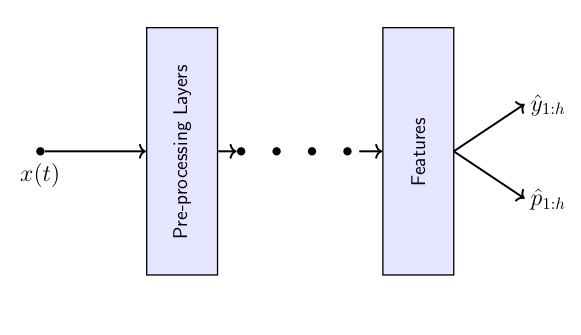
\includegraphics[width=0.5\textwidth]{figures/network.jpg}}
%\vspace{.3in}
%\caption{Network architecture}
%\label{fig:network}
%\end{figure}


In section \ref{sec:exp}, we use fully connected neural architectures having a maximum depth of 
two hidden layers, for prediction of outputs and time lags.

\section{Experiments}\label{sec:exp}


Just as the MNIST, CIFAR Santa Fe Laser and other data sets serve as a way to evaluate machine learning 
algorithms, it is necessary to propose benchmark problems for \emph{causal dynamic time lag}.

This is particularly challenging given the nature of the CDT problem, although causal time lag 
relationships do exist in real world data sets (\cite{doi:10.1002/jgra.50429}, \cite{ZHOU2006195}), 
it is difficult to find data sets with time lag relationships explicitly annotated.

This barrier can be surpassed in turn by careful construction of synthetic data sets which incorporate 
dynamic time lag relationships between causes and effects with various complexity.

Synthetic data sets allow us to evaluate the accuracy of both, the output and time lag predictions of 
CDT models. To this end, we propose four benchmark tests, which are motivated by their connection 
to the solar wind prediction problem, but which we hope can become canonical examples in the area 
of CDT modelling.

\subsection{Data Generation}

We start by generating the time series $x(t) \in \mathbb{R}^8$, of size $4000$ 
(one copy for training and another for test), which represent the driving/causal forces in our system. 
This can be achieved with good flexibility using \emph{Stochastic Langevin Dynamics} as shown in 
equation \ref{eq:data}.

\begin{align}
 x(t+1) &= (1 - \tau) x(t) + \mathcal{N}(0, \sigma^2) \label{eq:data}\\
 y(t+\Delta(t)) &= \alpha ||x(t)||^2 \label{eq:outputs}
\end{align}

In equation \ref{eq:outputs} we define the output $y(.)$ as the square norm of the appropriately 
time lagged input, where $\Delta(t)$ determines the causal time lag relationship.

\subsection{Generating Predictions}

As described in section \ref{sec:model} above, for each input pattern $x(t)$, the model 
generates two sets of predictions, i.e. ${\hat{y}_i}$, output estimates and probabilities $\hat{p}_i$ 
for the time window $i \in [t+\ell, t+\ell+h)$ of width $h$. In all of the following benchmarks we set 
$\ell = 0$ and $h = 20$.

In order to evaluate the model predictions for the benchmarks, we choose the prediction $\hat{y}_j$ 
which has the highest probability of a causal link $j = {argmax}_{i} \ \hat{p}_i \ \ i \in [t+\ell, t+\ell+h)$. 
The predictions $(\hat{y}_j, j)$ can now be compared to their corresponding ground truth values 
$(y(t + \Delta(t)), \Delta(t))$. 

When generating predictions for temporally successive test patters $x'(t)$, it is possible that our 
model produces time gaps in the reconstruction of the test outputs $y'(t)$. This can happen due to 
departure from the assumptions outlined in section \ref{sec:formulation}. We can get around these 
gaps using linear interpolation.


\subsection{Benchmark Problems}\label{sec:benchmark}

Based on the above framework we construct four benchmark problems.

\begin{enumerate}
\item \textbf{Problem I} Constant Lag: \newline 
$\Delta(t) = k$

\item \textbf{Problem II} Constant Velocity $\alpha ||x(t)||^2 + c$; Fixed Distance $d$: 
\newline $\Delta(t) = d/(\alpha ||x(t)||^2 + c),\ \alpha = \frac{100}{8},\ d = 1000,\ c = 40$

\item \textbf{Problem III} Constant Acceleration $a$; Fixed Distance $d$: 
\newline $\Delta(t) = (\sqrt{\alpha^2||x(t)||^4 + 2ad} - \alpha||x(t)||^2)/a,\ \alpha = \frac{50}{8},\ a = 5,\ d = 1000$

\item \textbf{Problem IV} Softplus time lag: 
\newline $\Delta(t) = exp\left(||x(t)||^2\right)/\left(1 + exp(||x(t)||^2)\right)$

\end{enumerate}



\subsection{Results}

The results of the experiments of \ref{sec:benchmark} are evaluated using the following charts.

\begin{enumerate}
    \item Output-Time Lag charts: Since the output time lag relationship can be expressed in closed 
          form, we can visualize this relationship in the generated data sets and evaluate how well 
          the model is able to infer it.
    \item Error Scatter charts: Scatter plots of prediction error in velocity vs prediction error 
          in time lag. They help in visualizing the shape of the error distribution.
\end{enumerate}


\subsubsection{Problem I}

This is the simplest of the benchmark problems, the task is simply to learn a constant time lag from 
the training data. On the test data set for this problem, the model predicts the correct time lag for 
$99.92\%$ of the samples. 

With respect to prediction of the outputs, the model has a \emph{mean absolute error} (MAE) of 
$6.904677$ and achieves a Pearson correlation coefficient of $0.9795$ on a test data set in which the 
output lies in the range $[9.454, 290.550]$. It should be noted that the $y(t - 1)$ predictor 
achieves a MAE of $5.186521$ and a Pearson correlation of $0.991$ on this data set. The model is 
thus able to learn the input-output and time lag mappings easily for this problem.

\begin{figure}[h]
\vspace{.3in}
\centerline{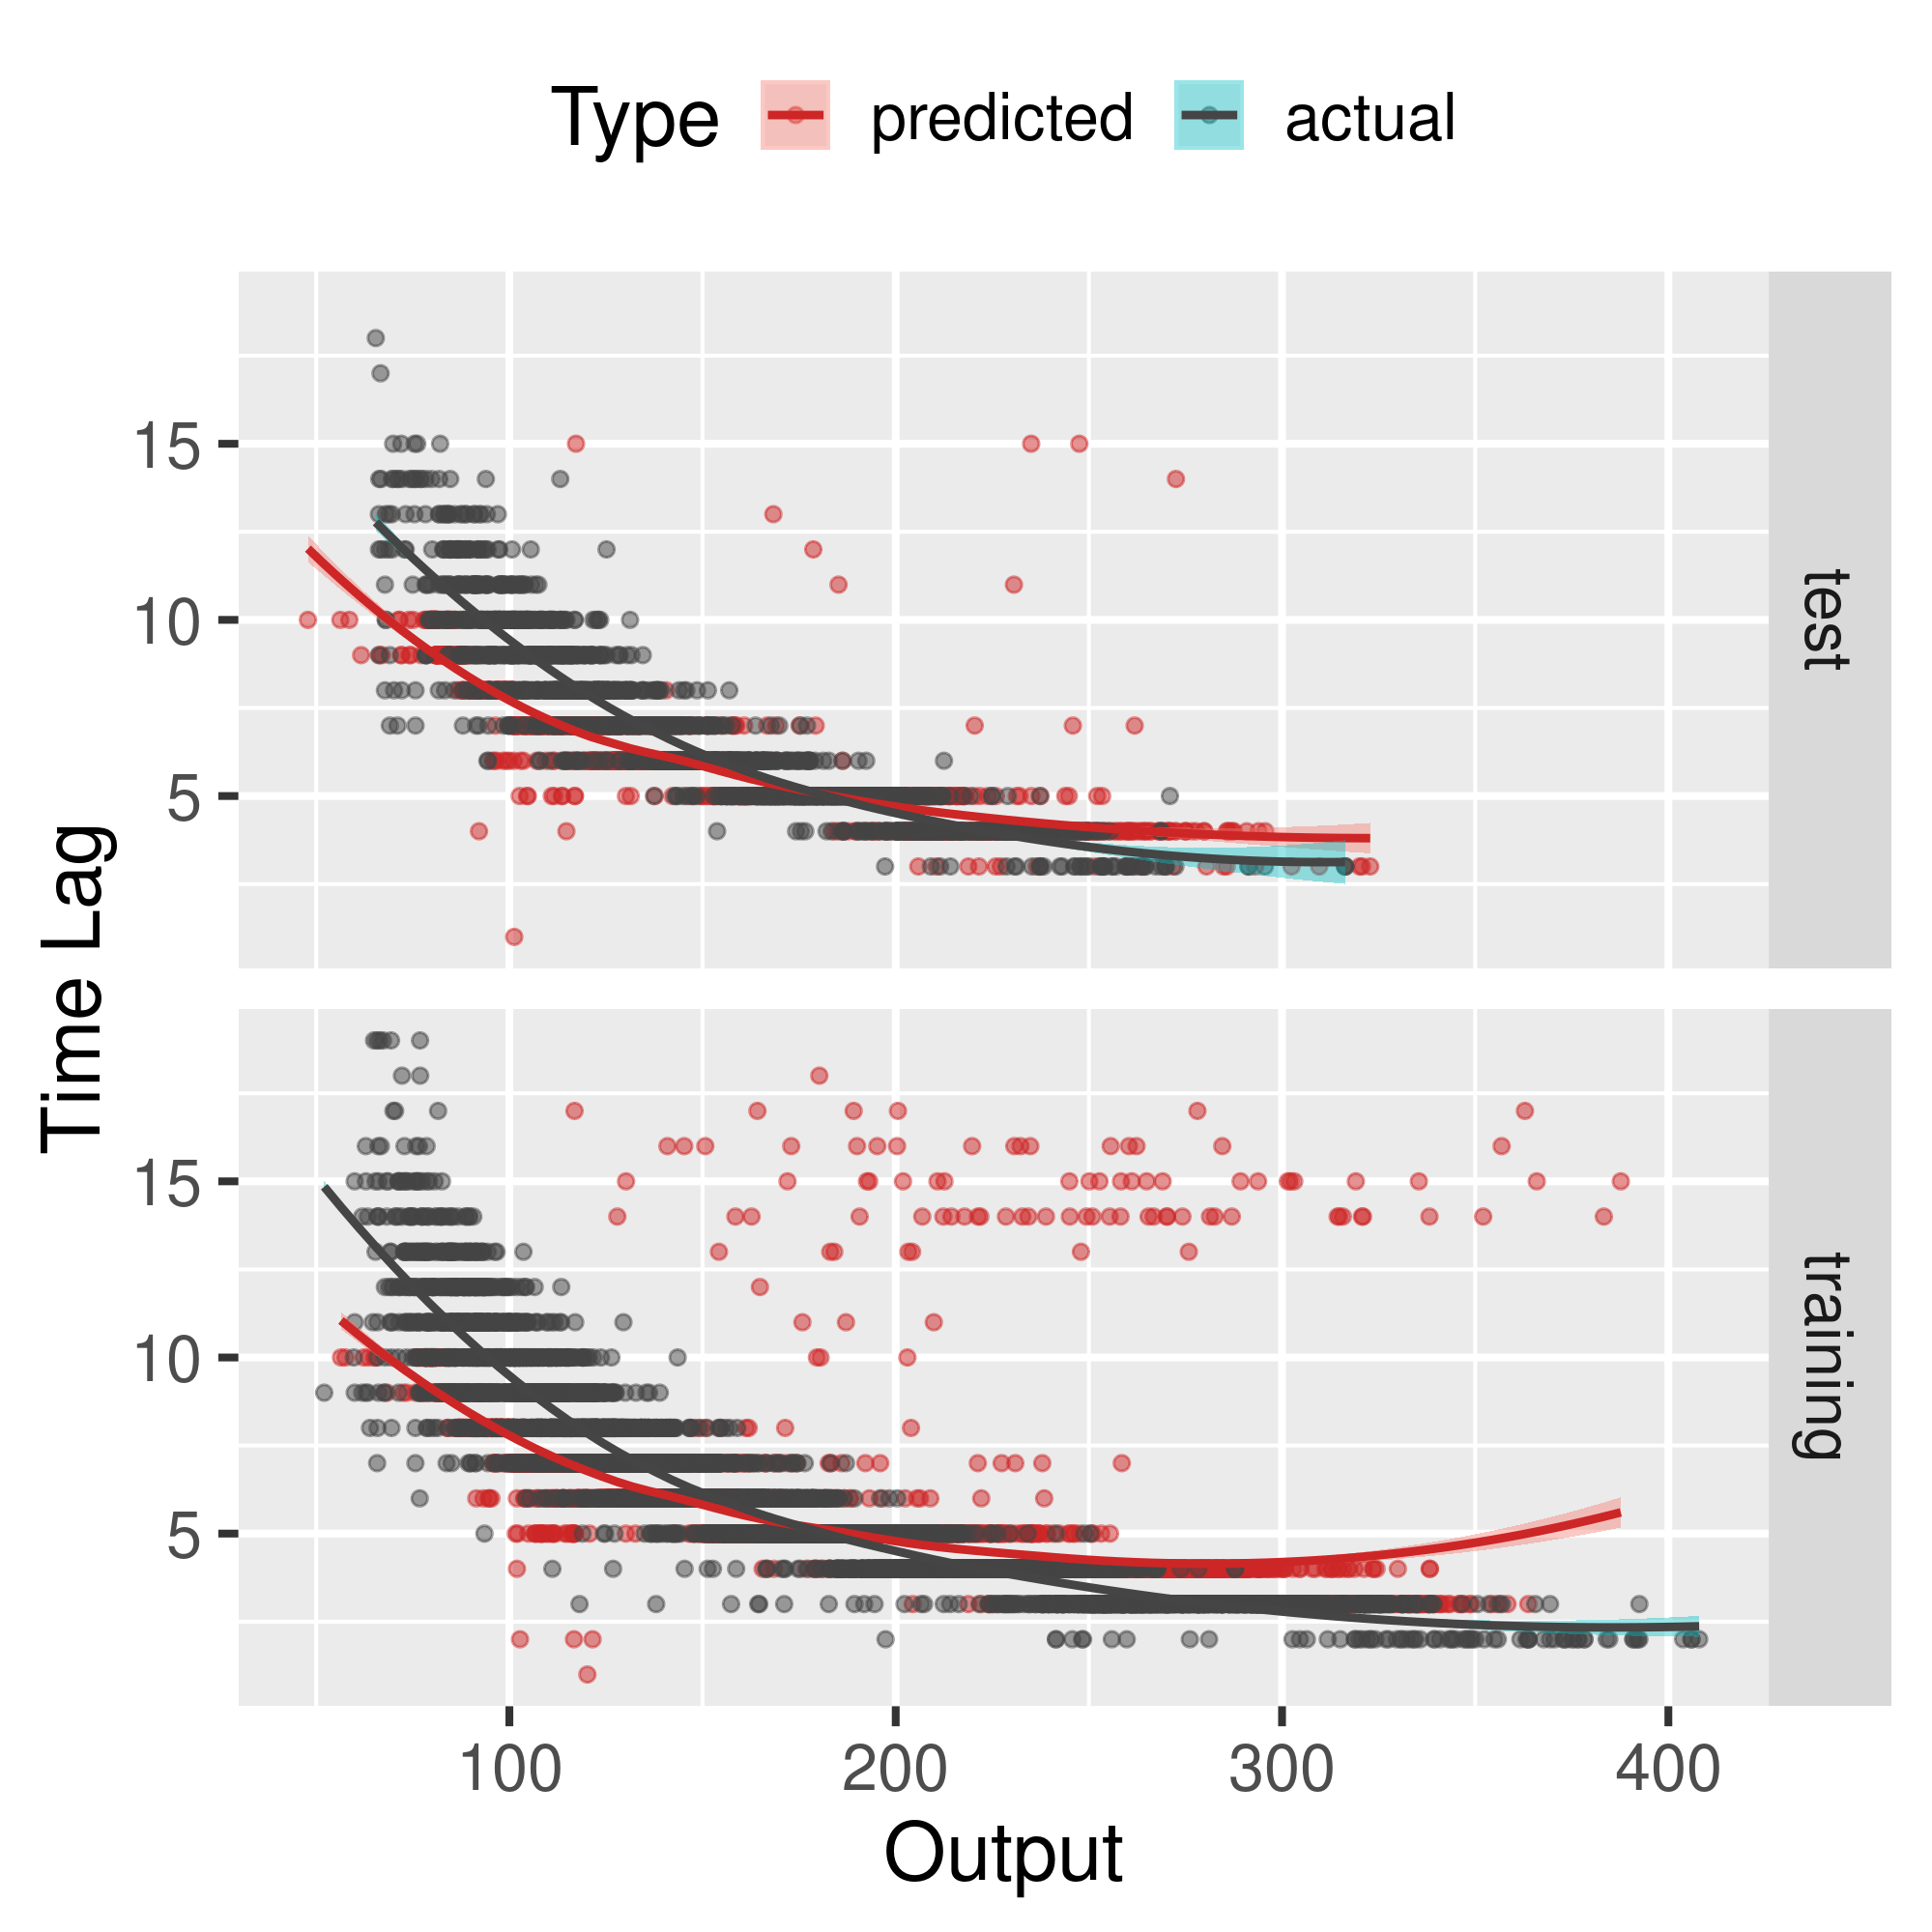
\includegraphics[width=0.5\textwidth]{figures/exp2_scatter_v_tl.png}}
\vspace{.3in}
\caption{\textbf{Problem II}, Output-Time Lag Scatter plot on test data; model predictions in red and actual data in black}
\label{fig:problem2_scatter}
\end{figure}

\begin{figure}[h]
\vspace{.3in}
\centerline{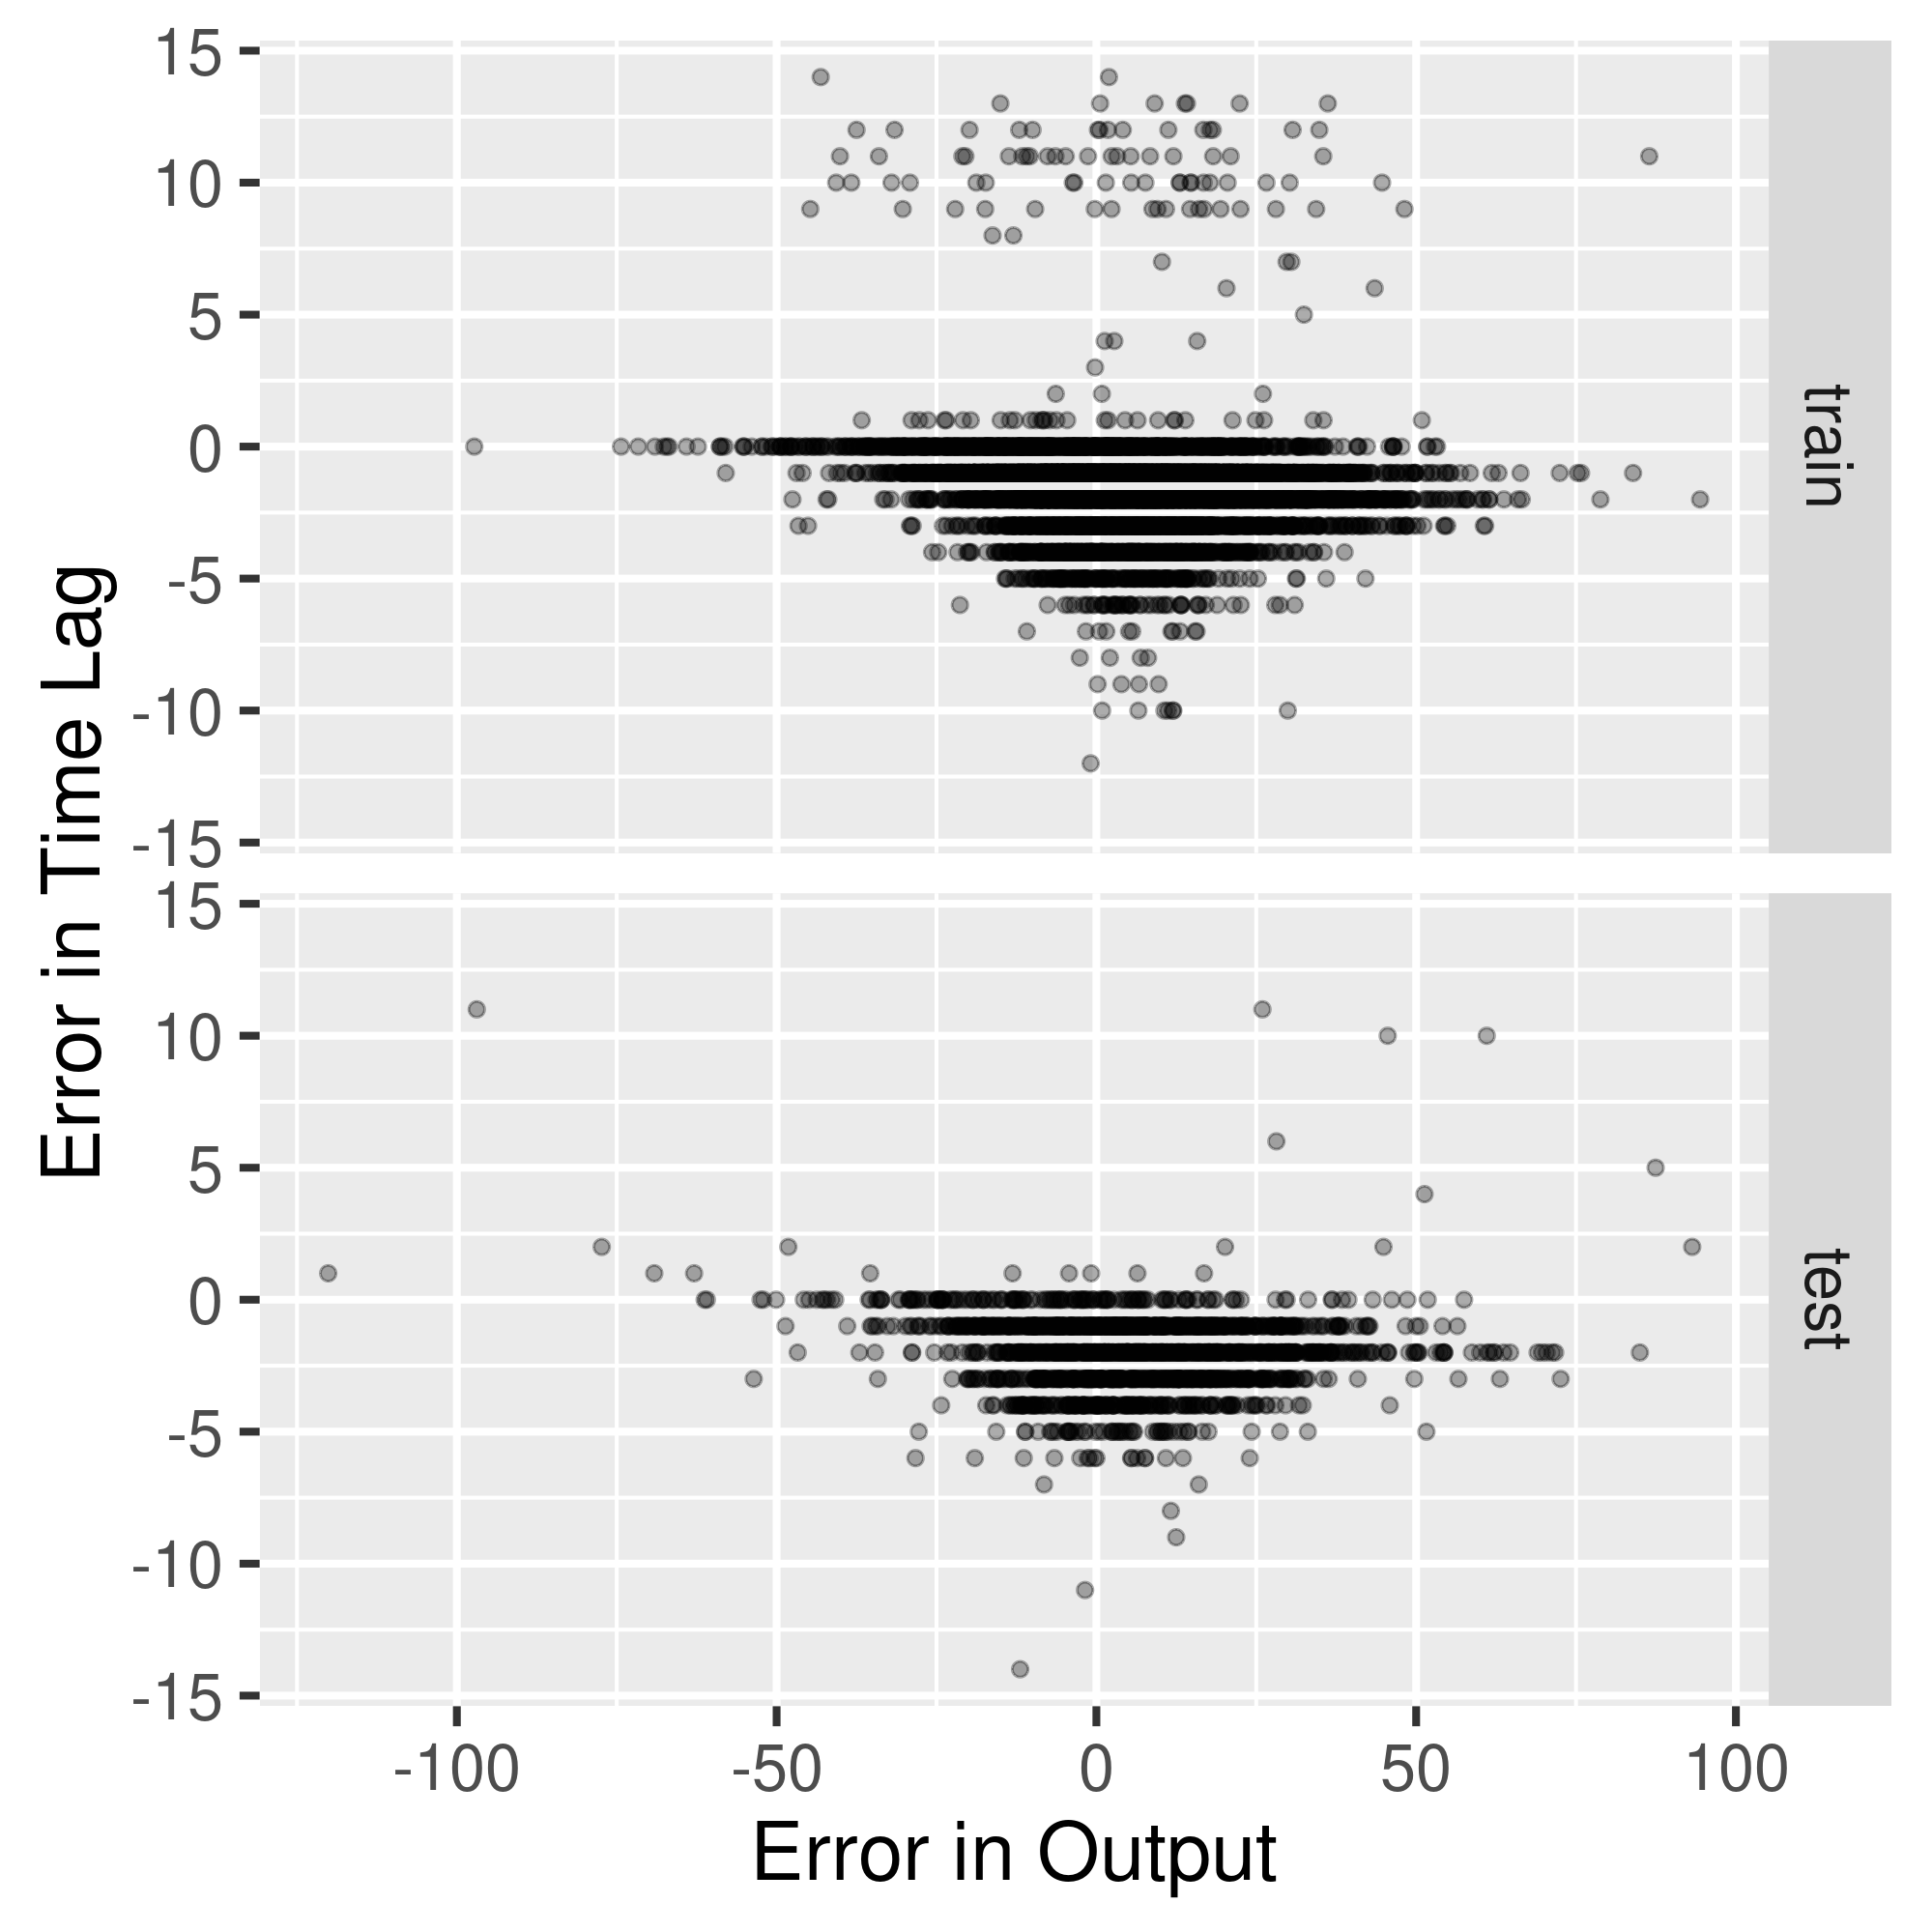
\includegraphics[width=0.5\textwidth]{figures/exp2_scatter_errors.png}}
\vspace{.3in}
\caption{\textbf{Problem II}, Error in prediction of output vs error in time lag prediction}
\label{fig:problem2_error}
\end{figure}


\begin{figure}[h]
\vspace{.3in}
\centerline{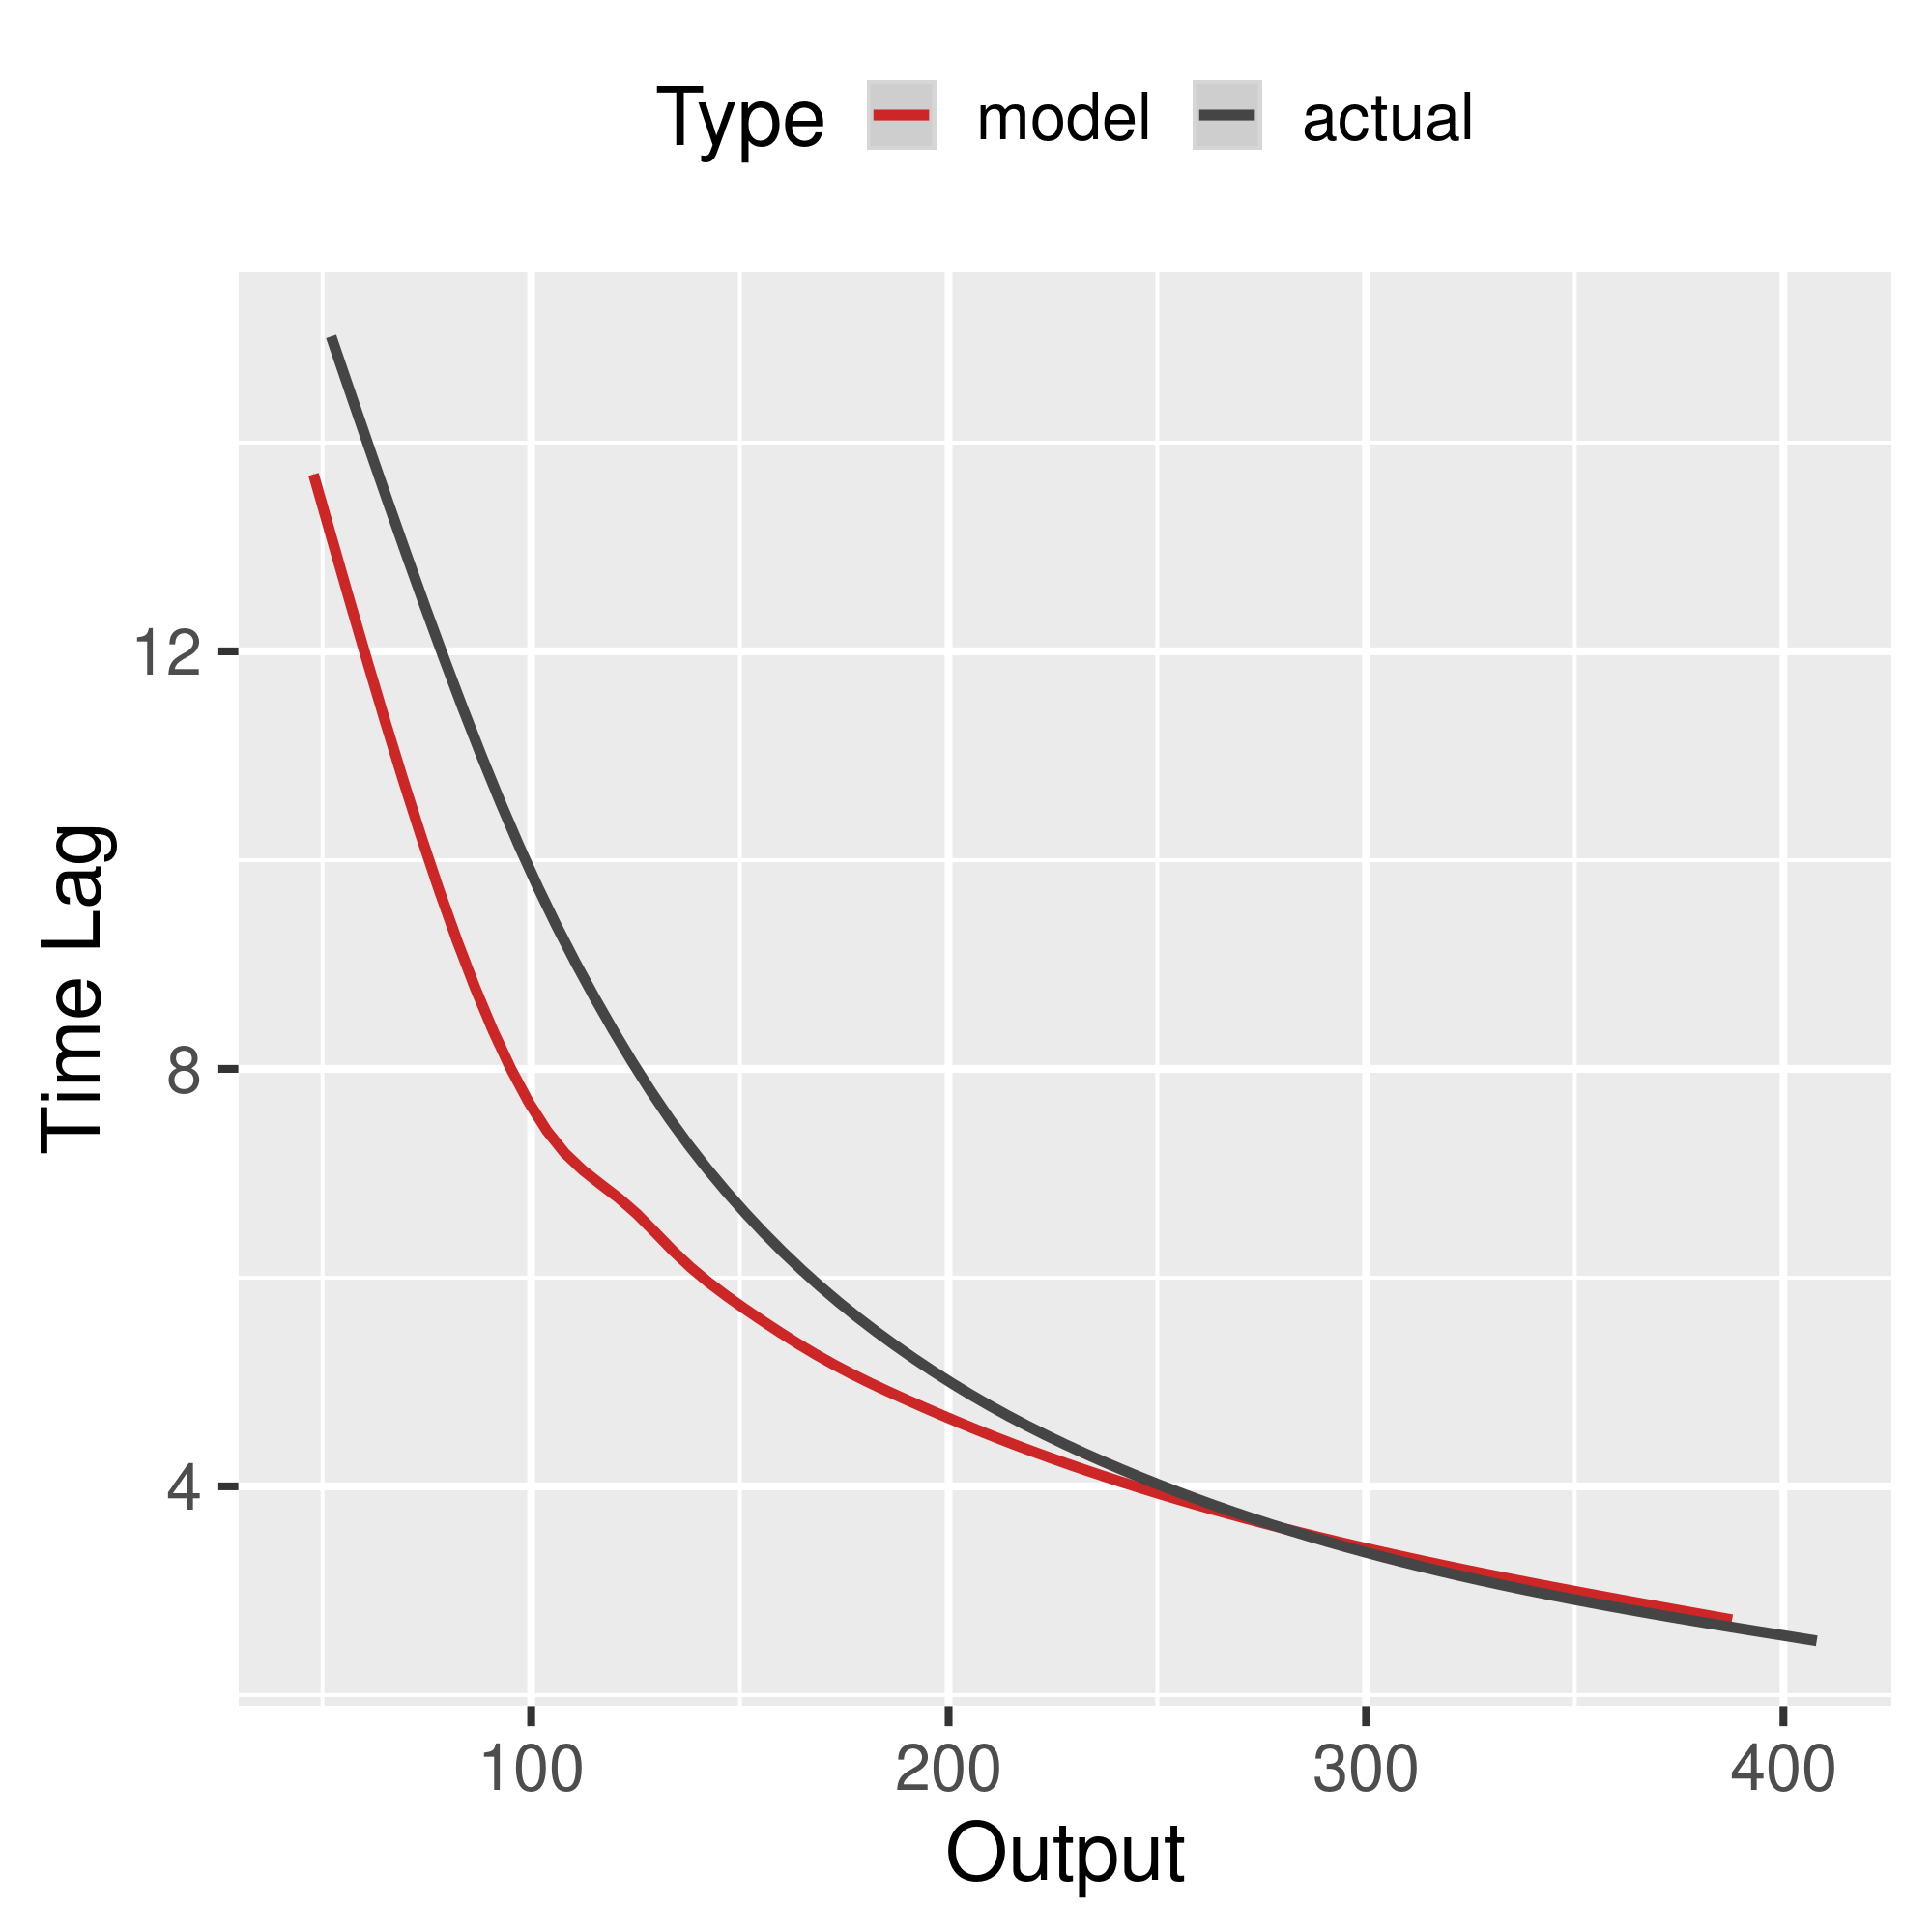
\includegraphics[width=0.5\textwidth]{figures/exp2_predictive_curves.png}}
\vspace{.3in}
\caption{\textbf{Problem II}, Output vs Time Lag Relationship}
\label{fig:problem2_curves}
\end{figure}

\begin{figure}[h]
\vspace{.3in}
\centerline{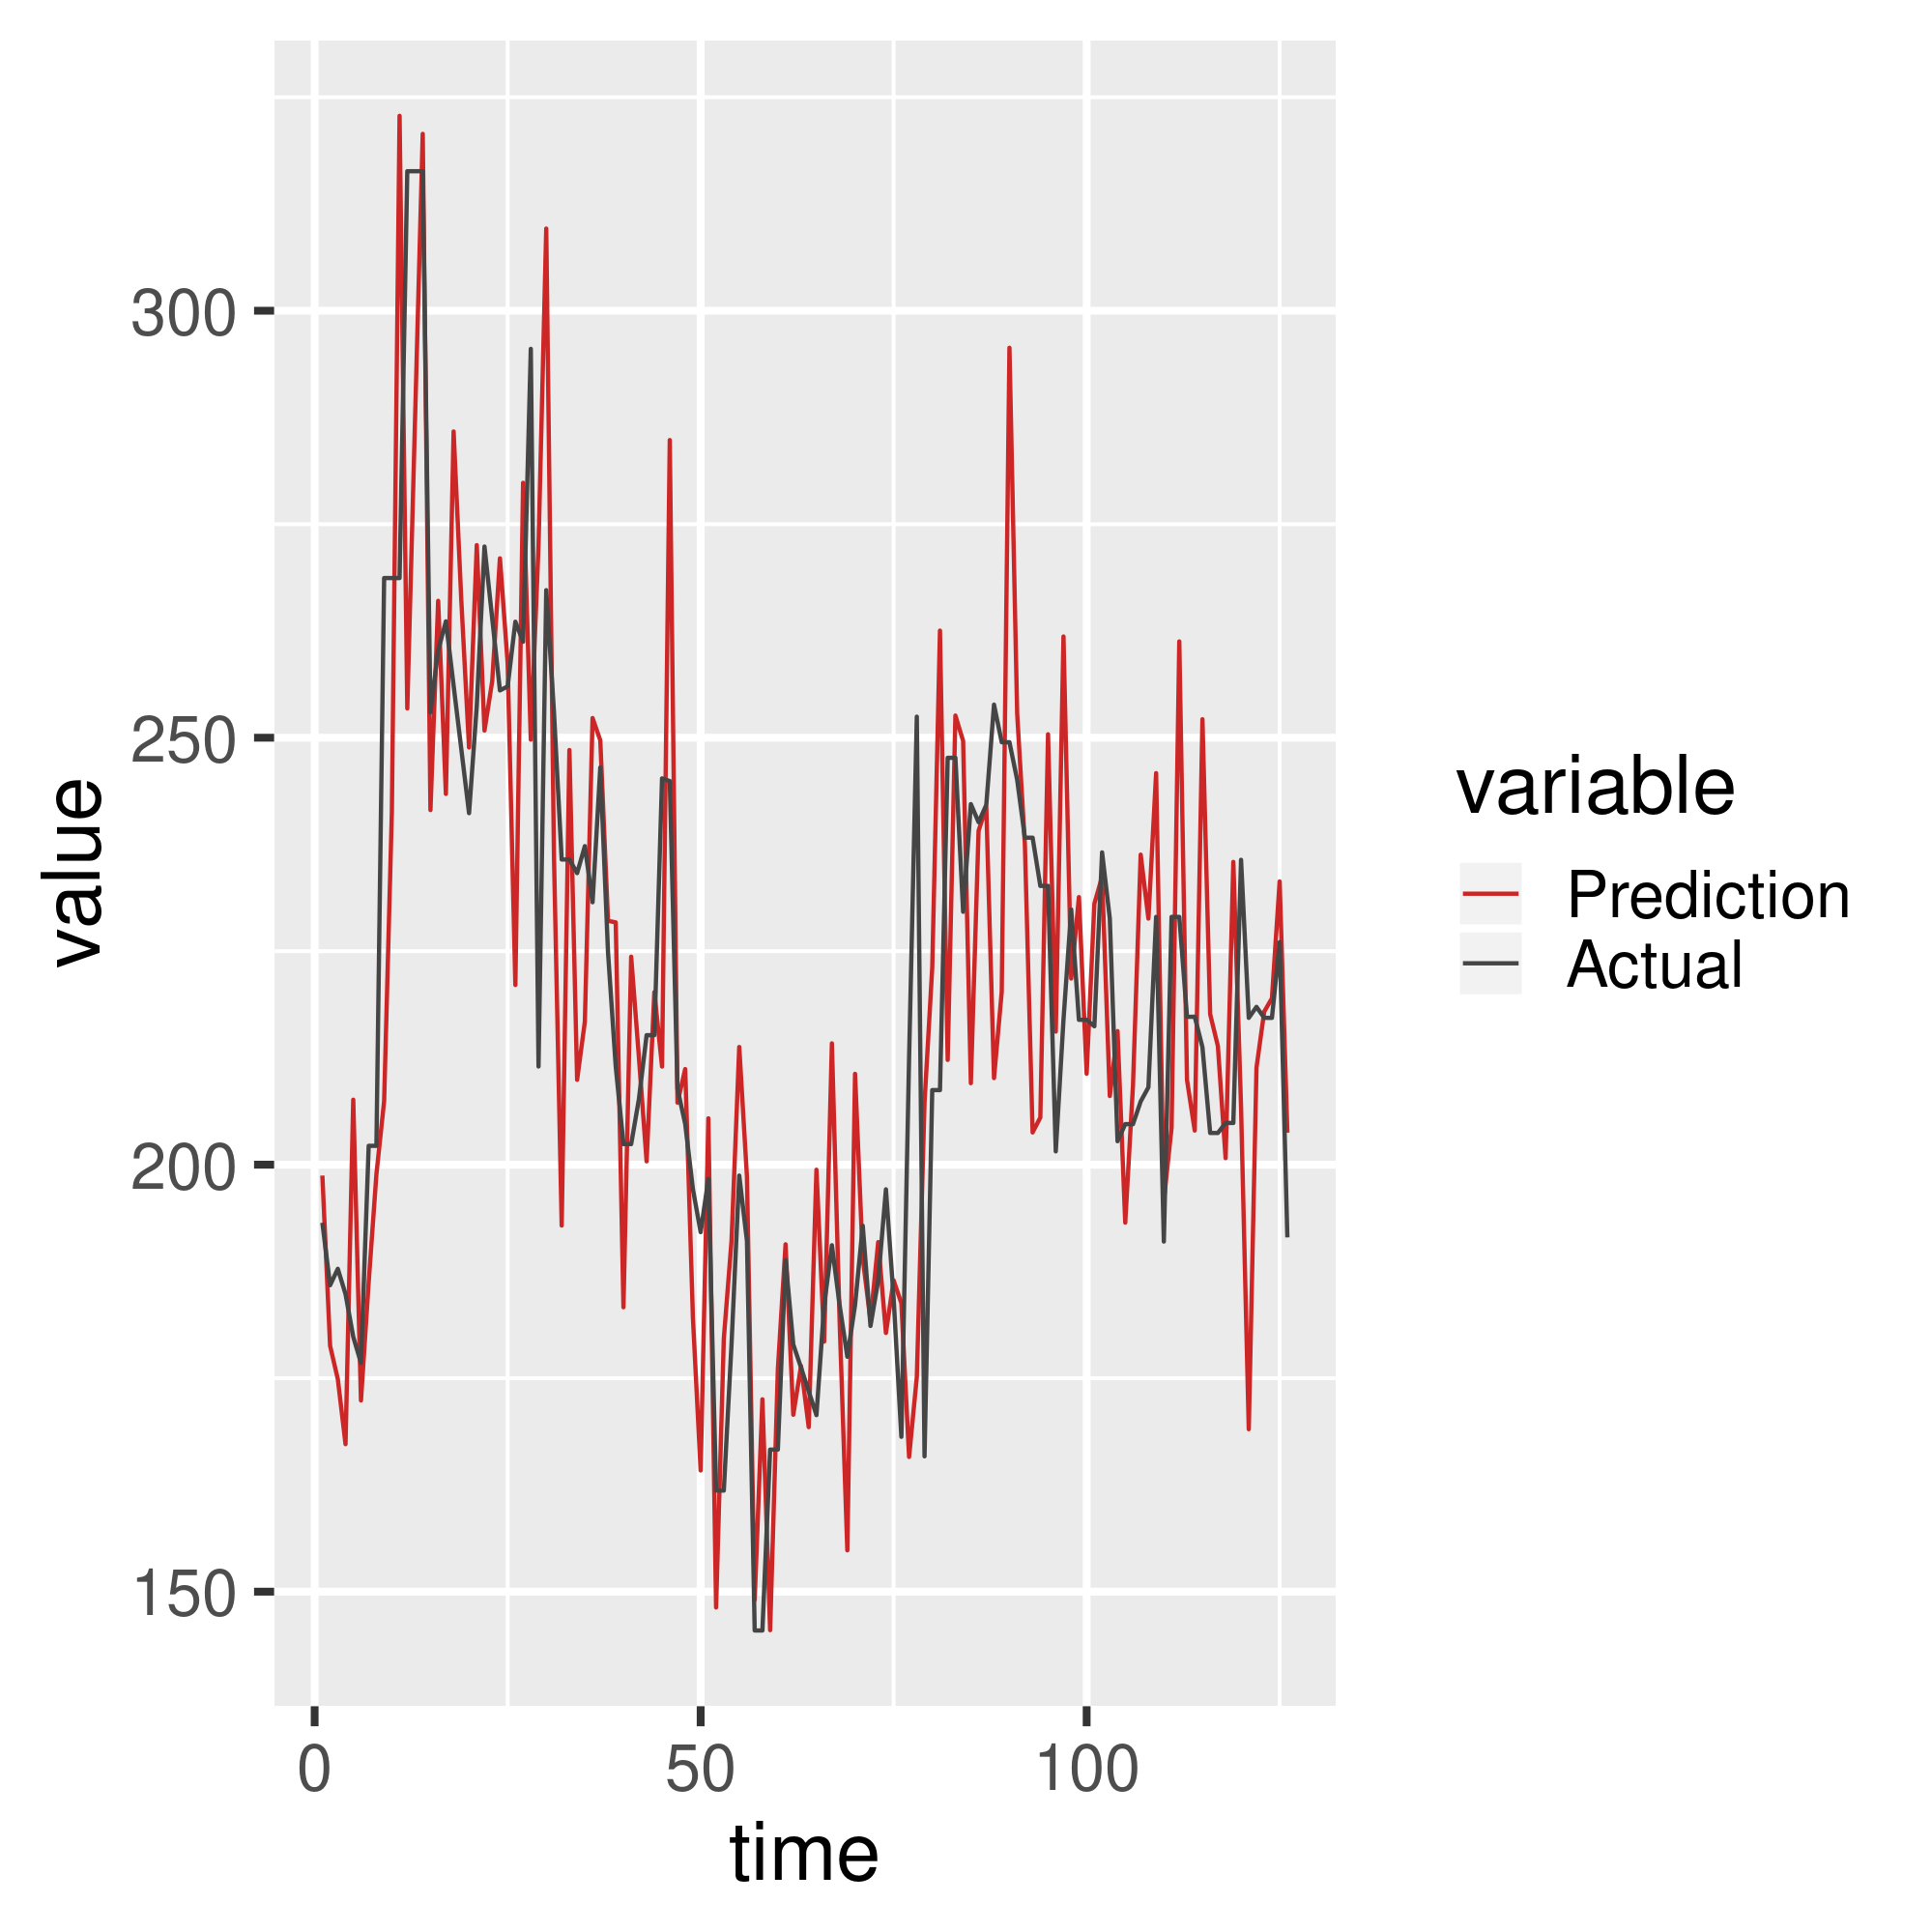
\includegraphics[width=0.5\textwidth]{figures/exp2_timeseries_pred.png}}
\vspace{.3in}
\caption{\textbf{Problem II}, A portion of the test time series reconstructed using the model}
\label{fig:problem2_timeseries}
\end{figure}


\subsubsection{Problem II}

Figure \ref{fig:problem2_scatter} shows a scatter plot between the output value and associated 
time lag, it compares the scatter distribution generated by the model and compares it with the 
distribution seen in the test data.

In figure \ref{fig:problem2_error} we present a scatter plot which shows the distribution of the 
errors in output versus the error in time lag predictions.

In figure \ref{fig:problem2_curves} we present smoothed trends extracted from the data presented in 
\ref{fig:problem2_scatter}, the red curve represents the output time lag function learned by the model 
while the black curve is the \emph{ground truth} dependence between the two. 

We can see that the model is able to approximate the inverse relationship between the output and 
time lag from the training data.

\begin{figure}[h]
\vspace{.3in}
\centerline{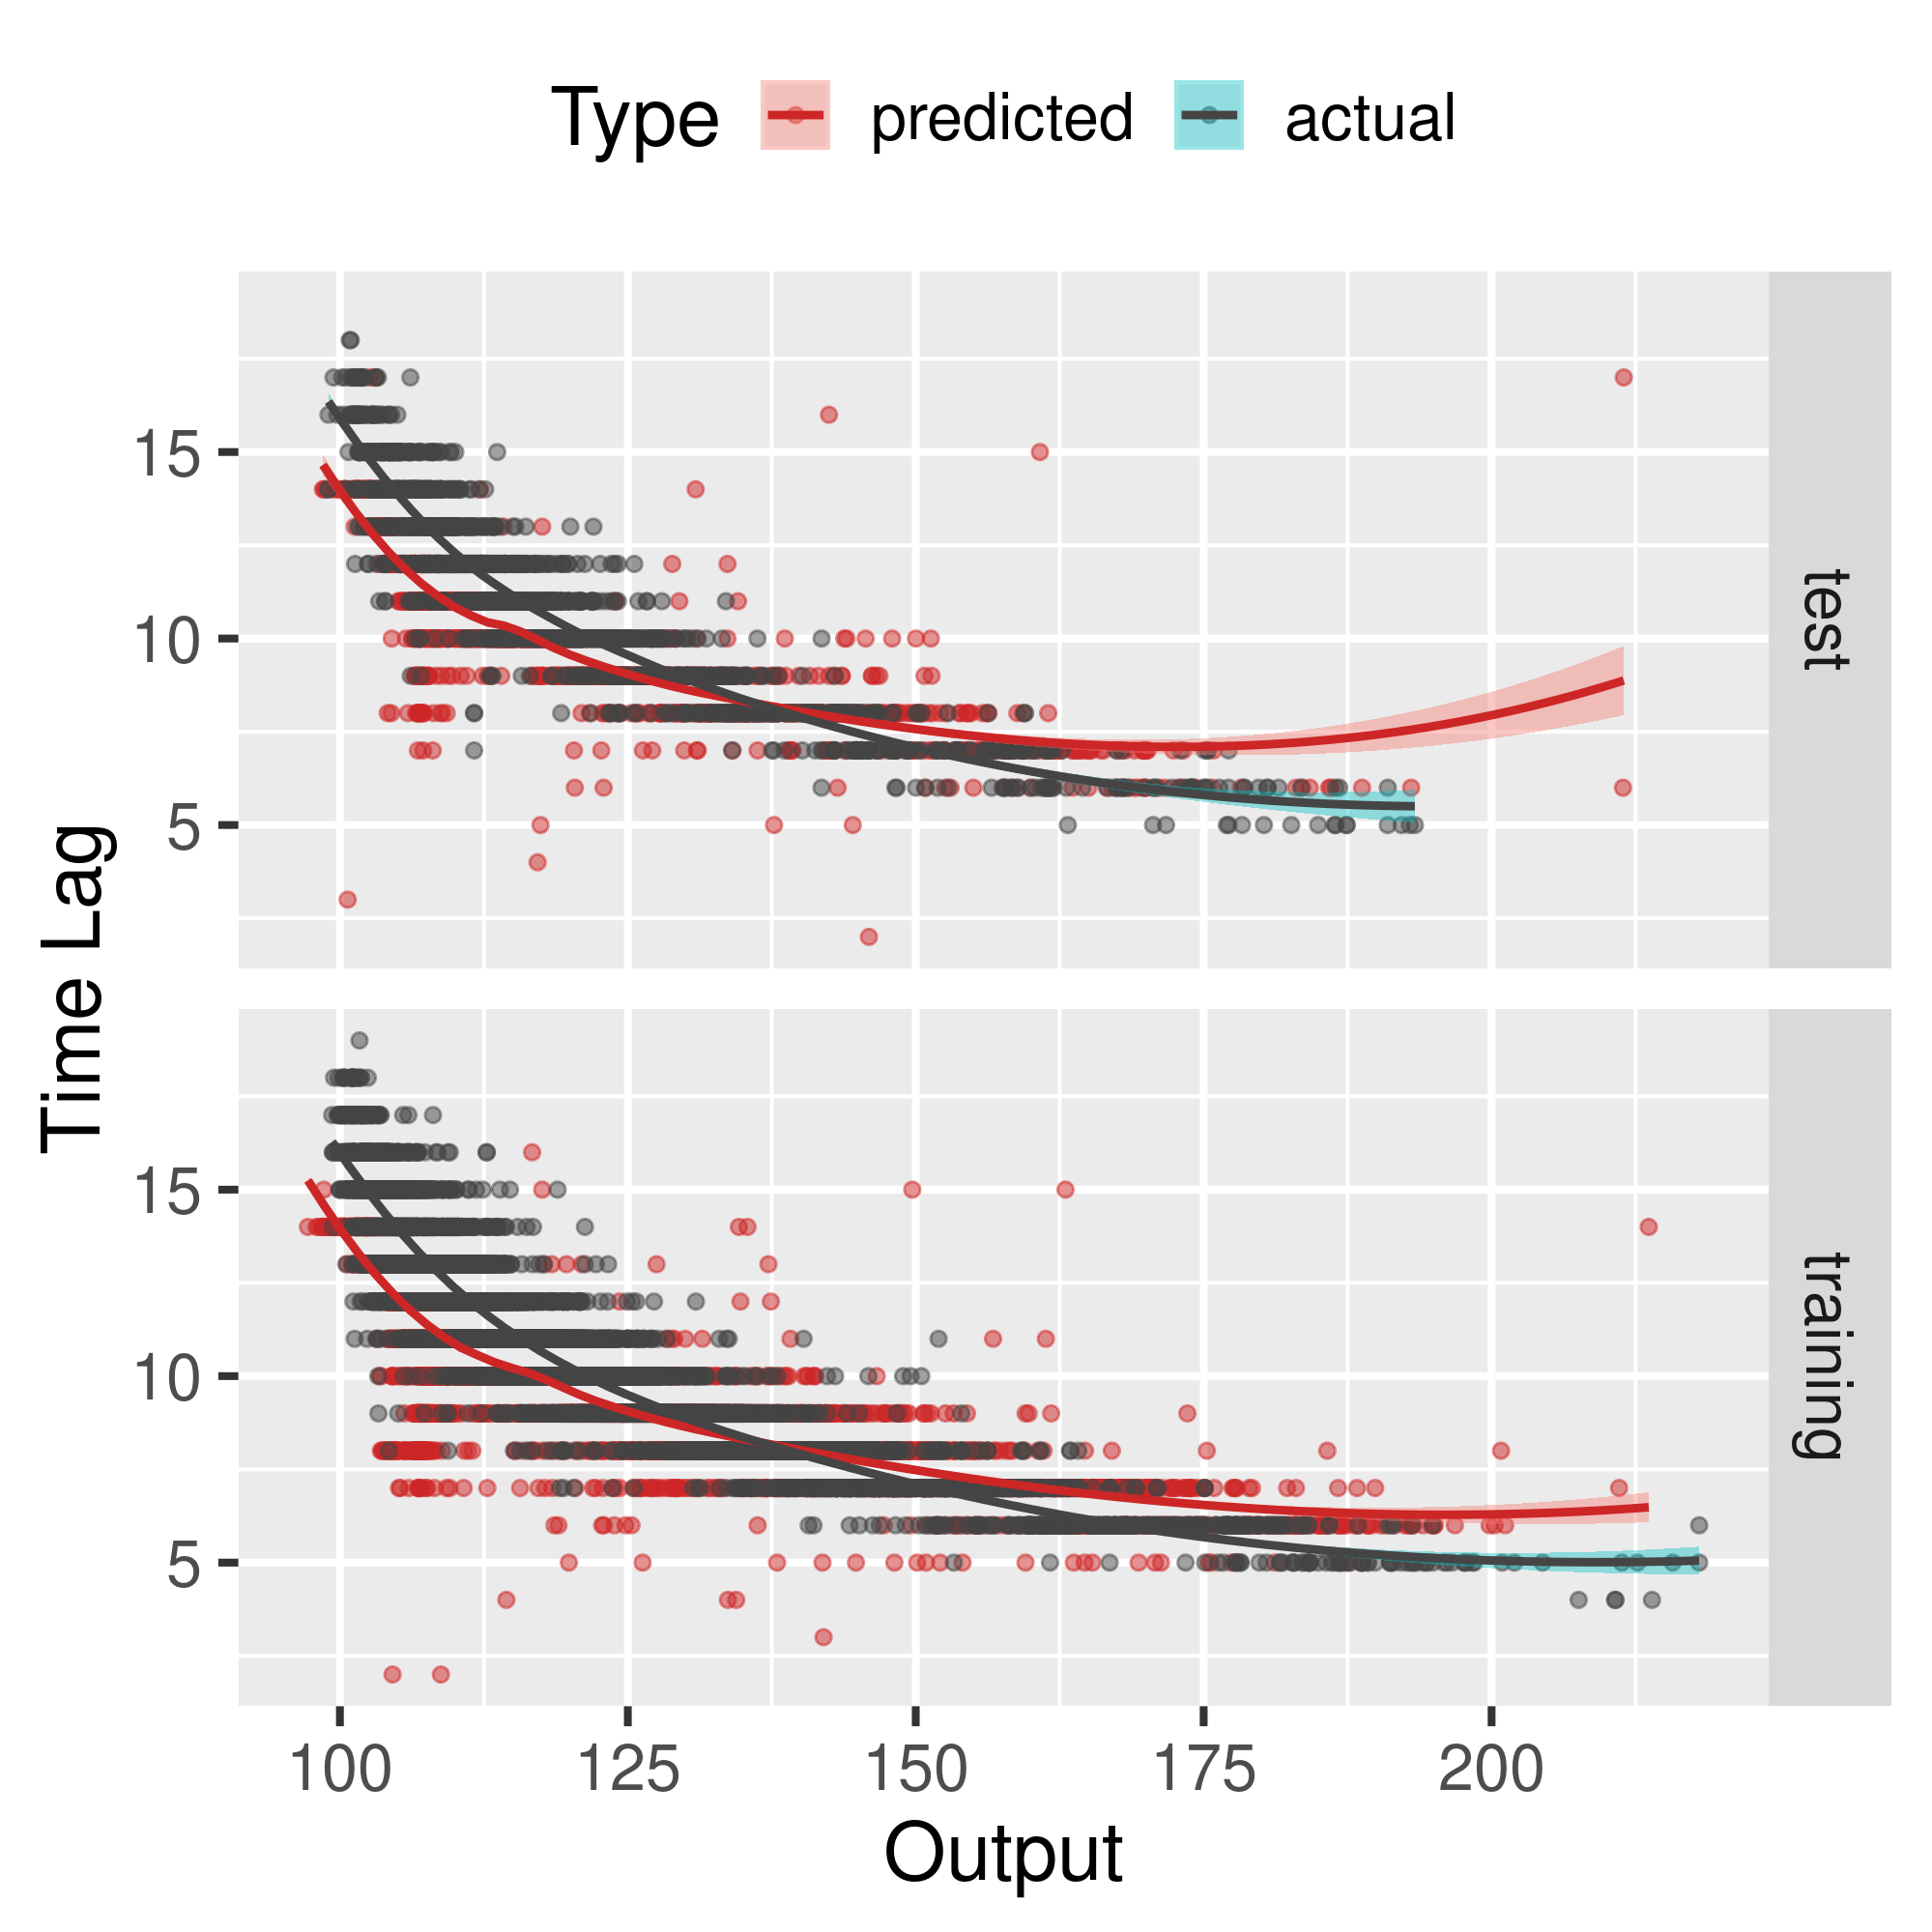
\includegraphics[width=0.5\textwidth]{figures/exp3_scatter_v_tl.png}}
\vspace{.3in}
\caption{\textbf{Problem III}, Output-Time Lag Scatter plot; model predictions in red and actual data in black}
\label{fig:problem3_scatter}
\end{figure}

\begin{figure}[h]
\vspace{.3in}
\centerline{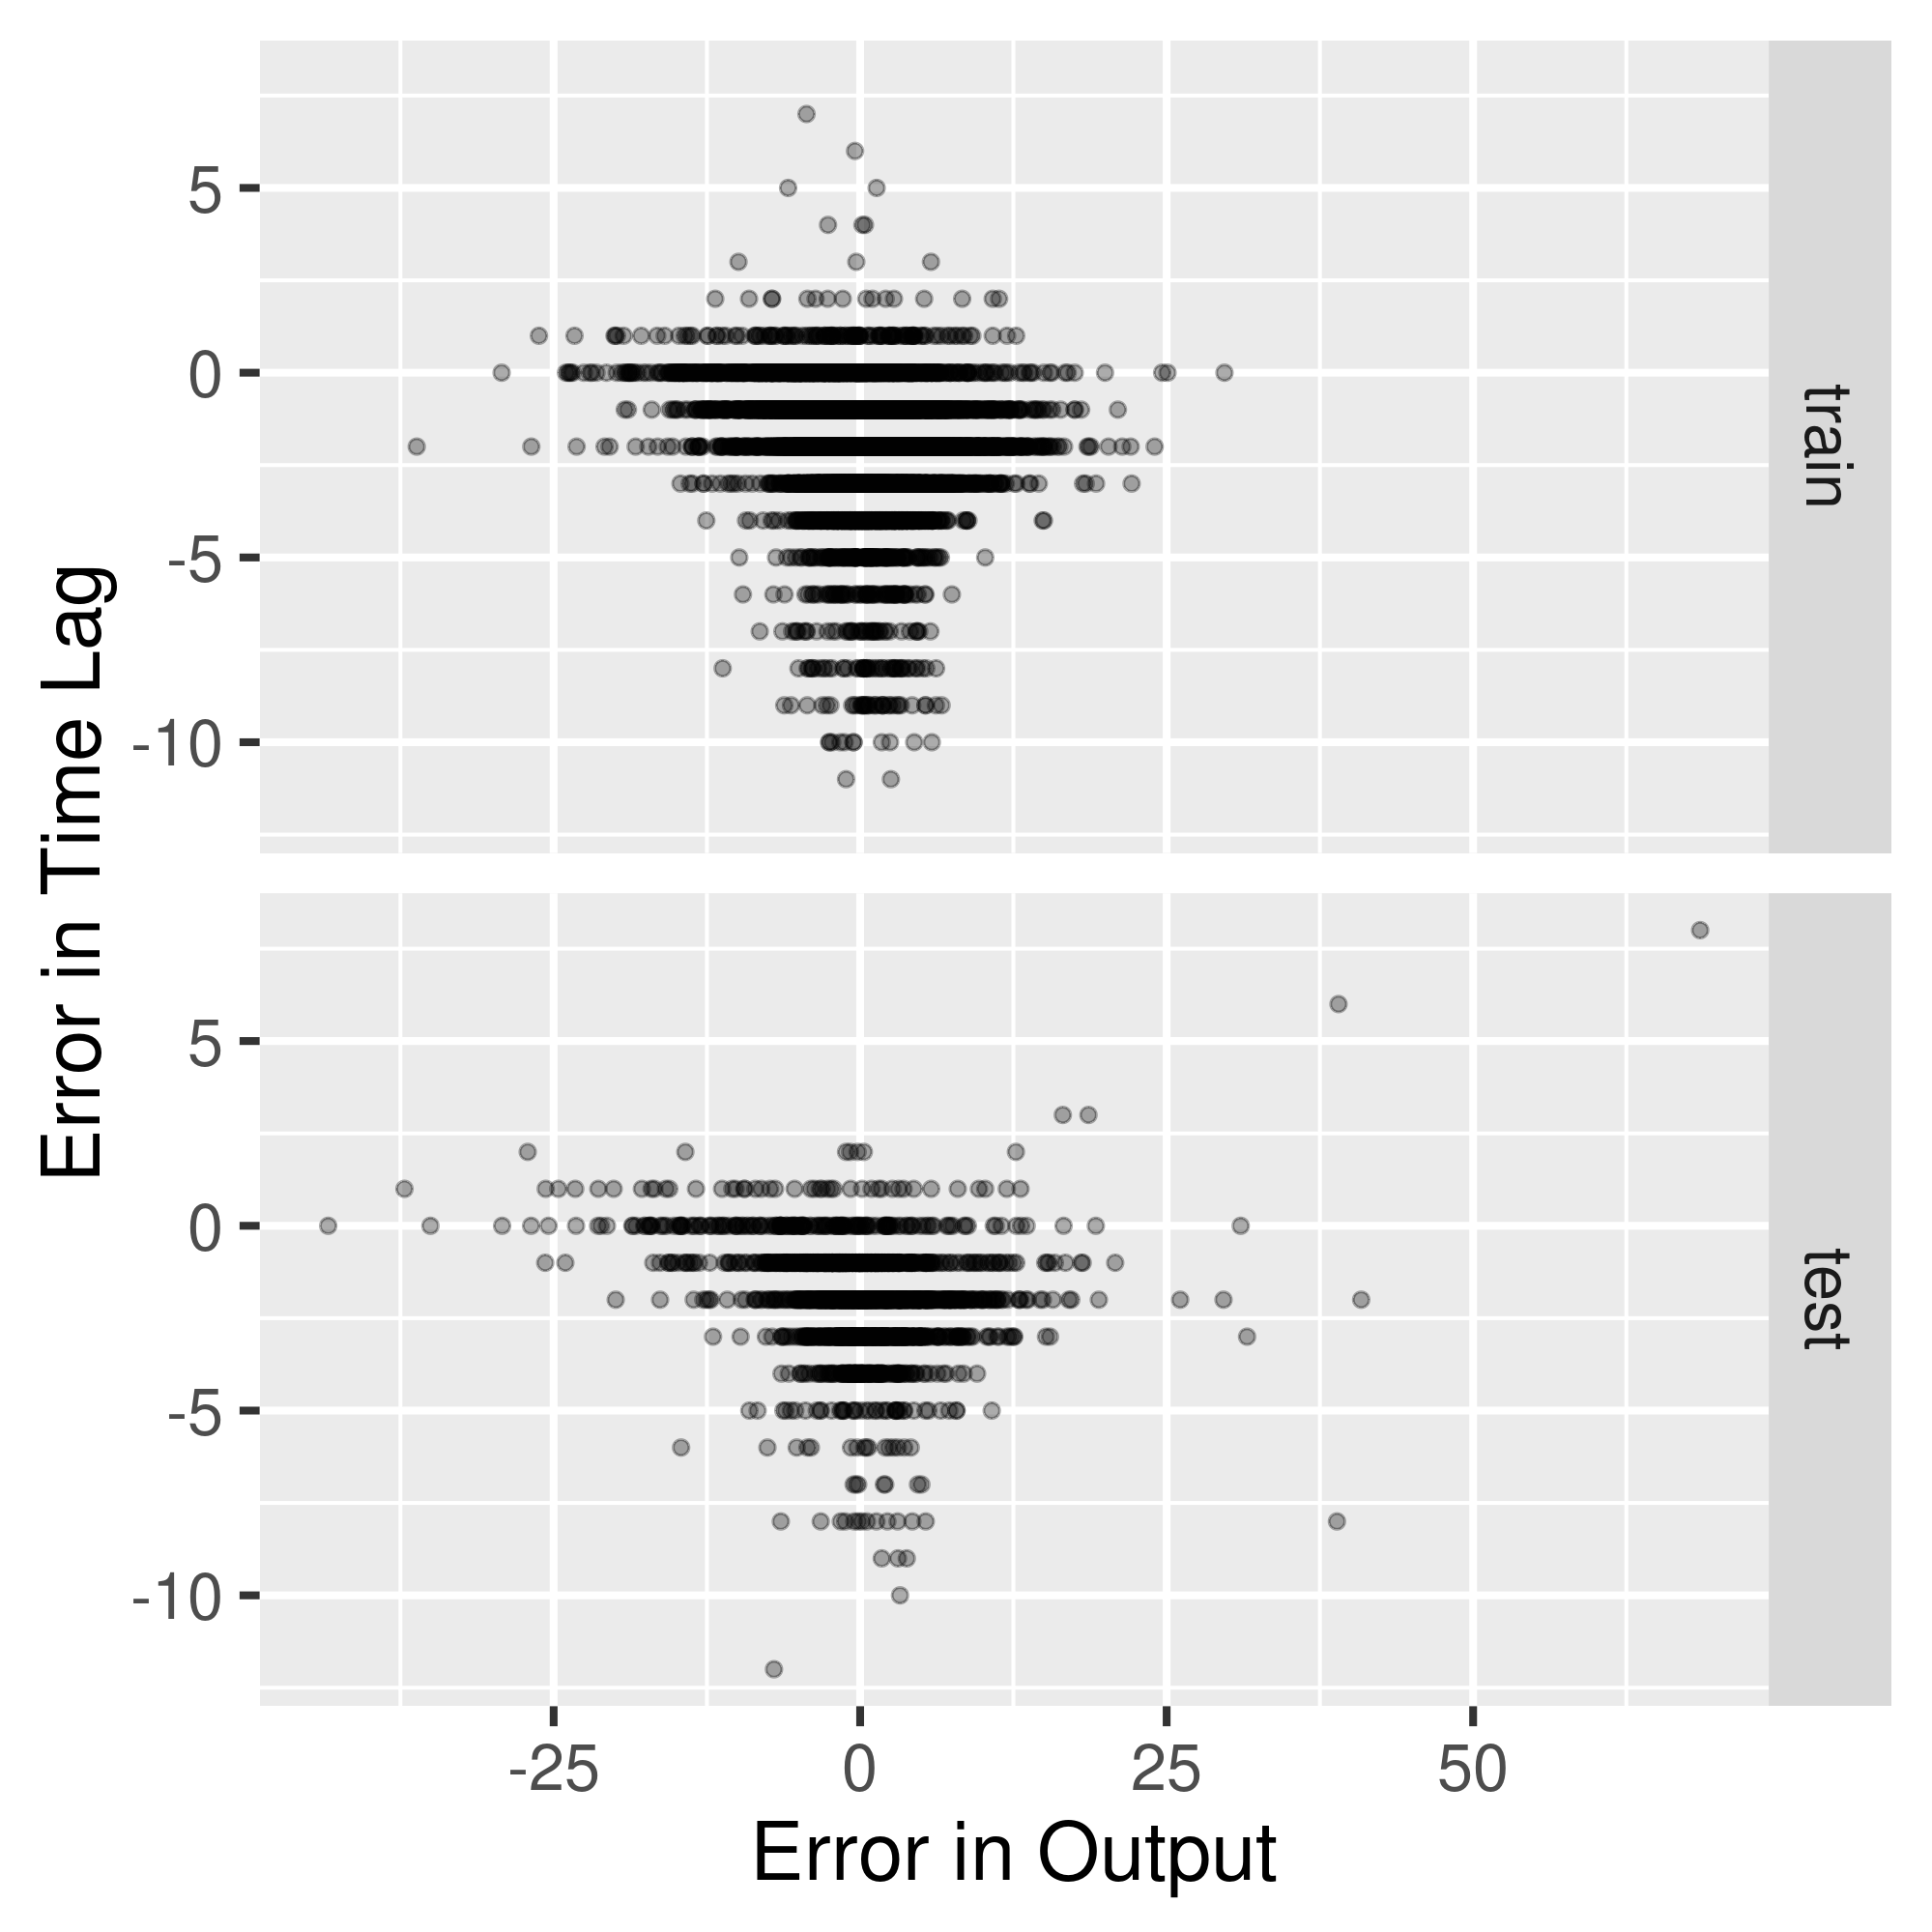
\includegraphics[width=0.5\textwidth]{figures/exp3_scatter_errors.png}}
\vspace{.3in}
\caption{\textbf{Problem III}, Error in prediction of output vs error in time lag prediction}
\label{fig:problem3_error}
\end{figure}

\begin{figure}[h]
\vspace{.3in}
\centerline{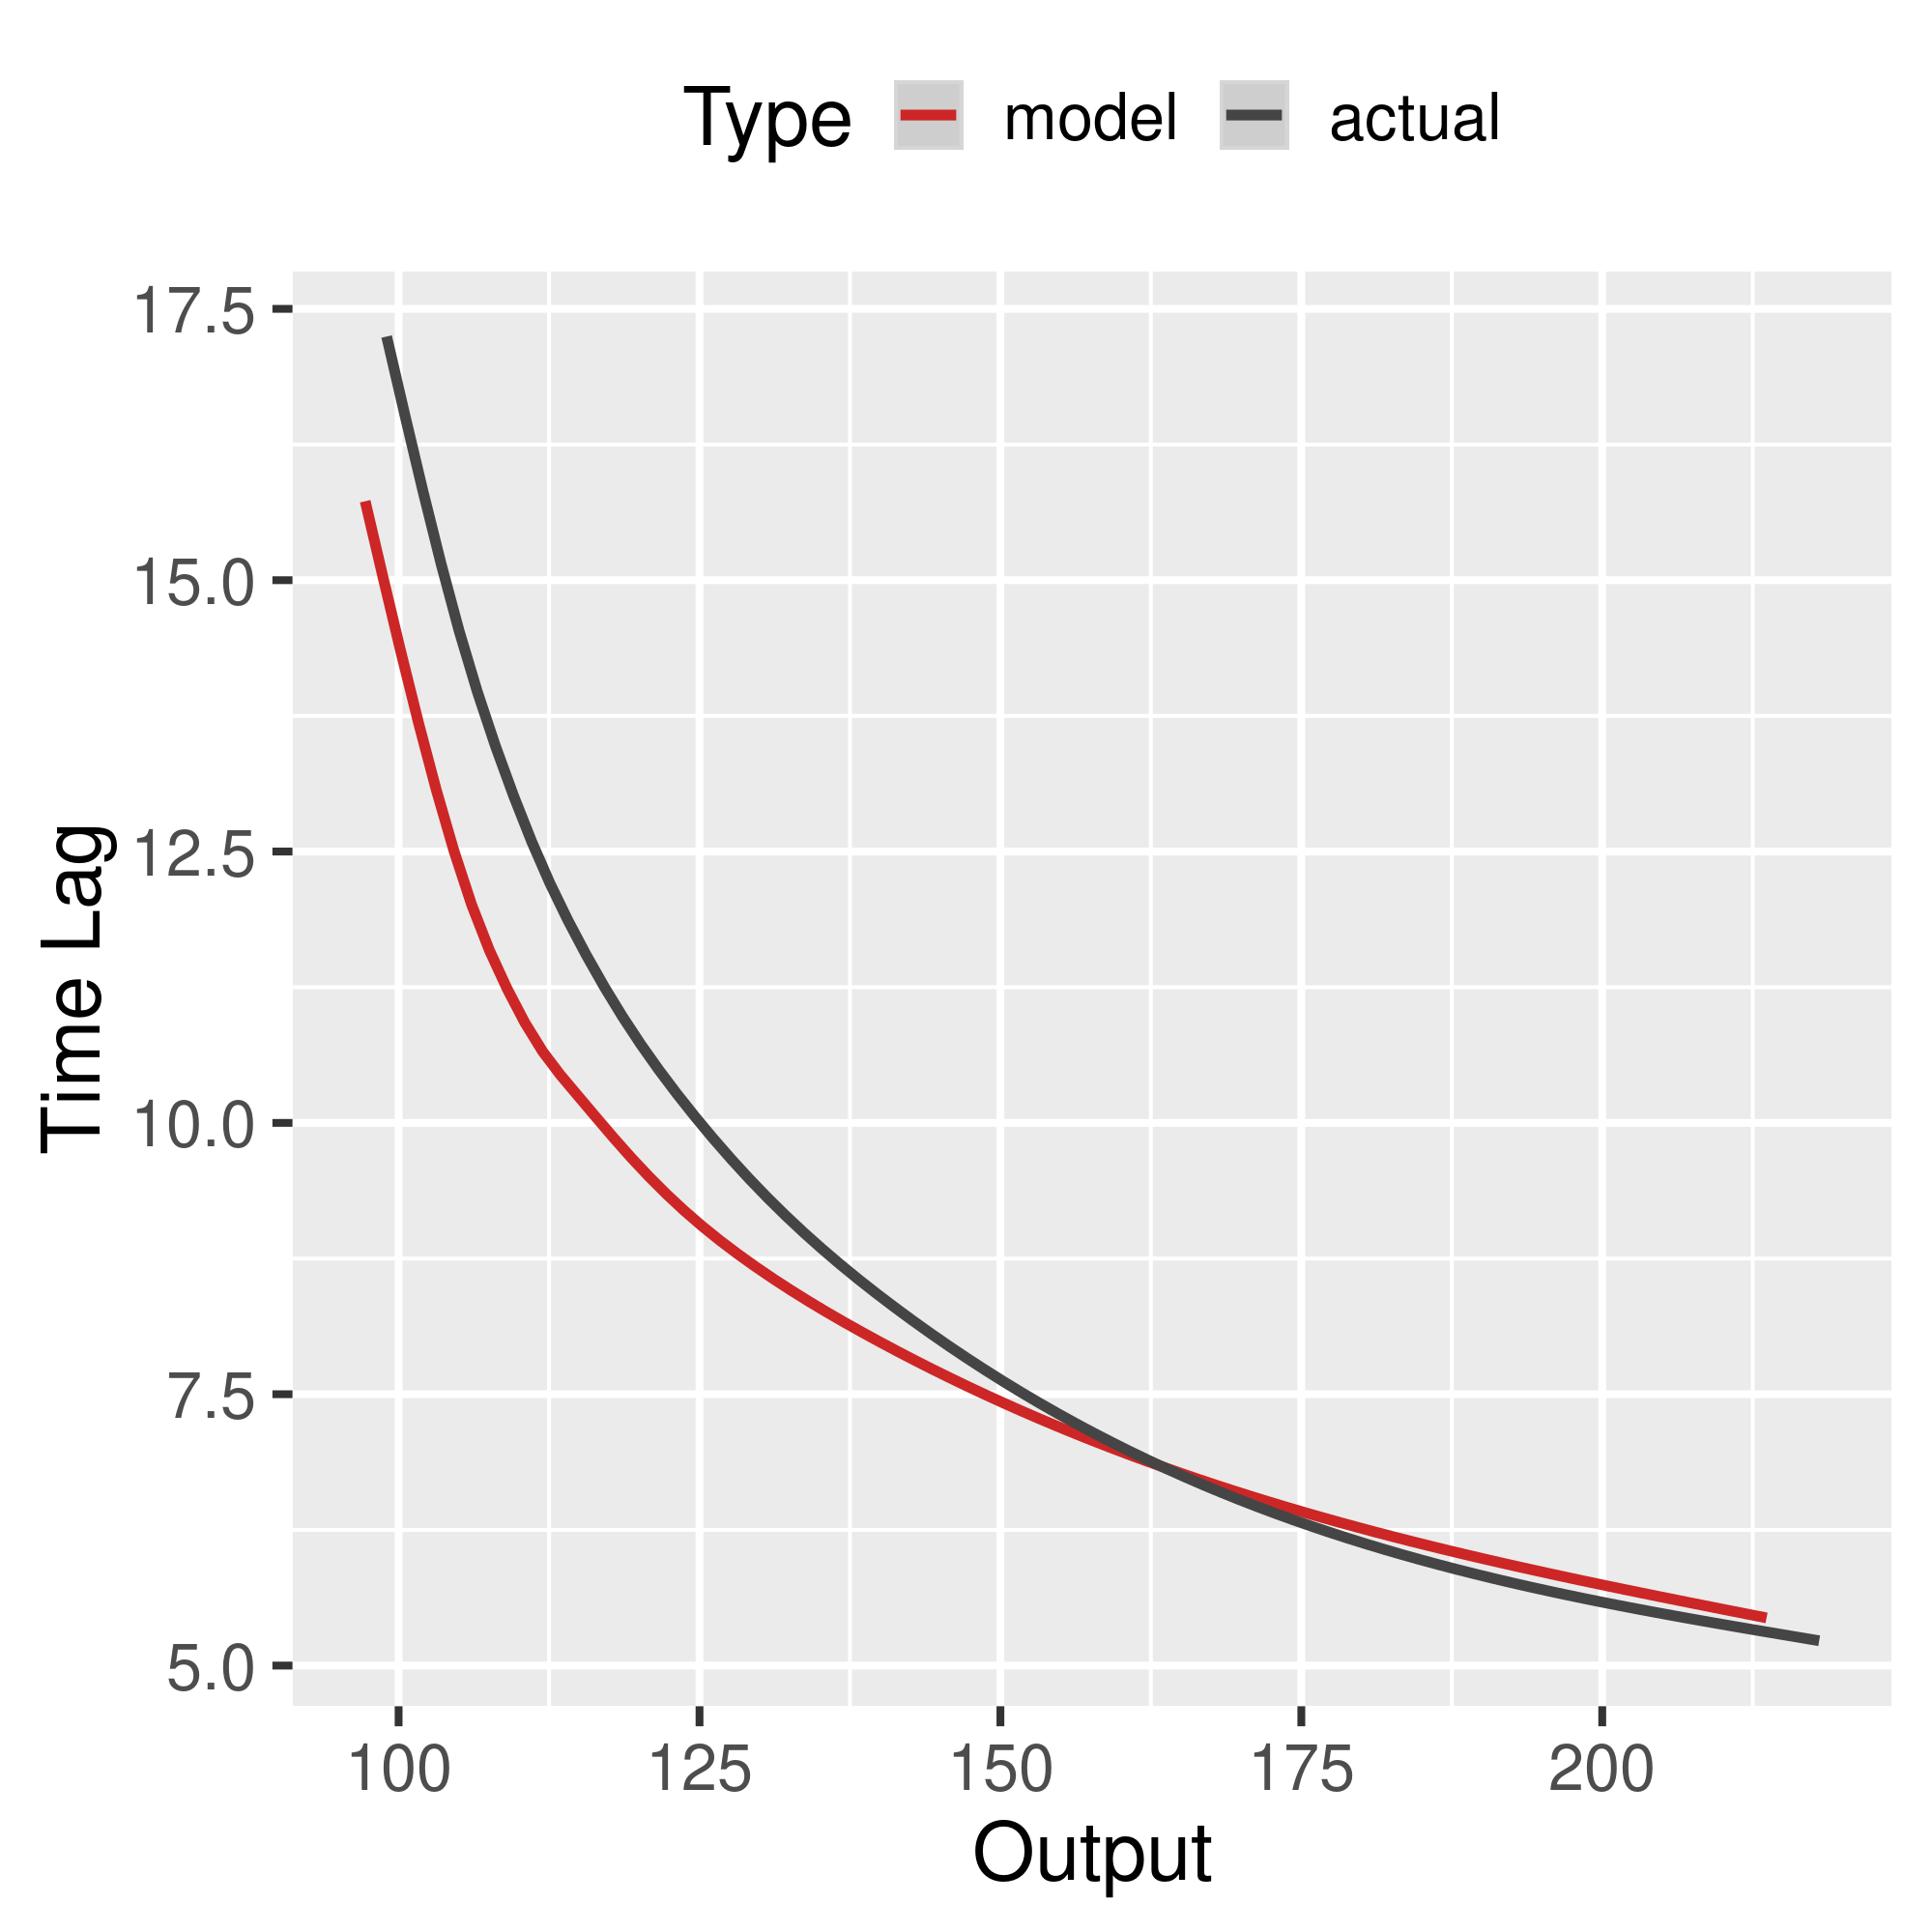
\includegraphics[width=0.5\textwidth]{figures/exp3_predictive_curves.png}}
\vspace{.3in}
\caption{\textbf{Problem III}, Output vs Time Lag Relationship}
\label{fig:problem3_curves}
\end{figure}


\subsubsection{Problem III}

Problem III involves a more complicated output time lag relationship than problem II due to the 
effect of acceleration. From figures \ref{fig:problem3_scatter} and \ref{fig:problem3_error}, 
it can be observed that the model can still learn the time lag and output mappings although 
in this case the time lag error distribution has a slightly longer tail in figure 
\ref{fig:problem3_error} as compared to \ref{fig:problem2_error}.

One observation common to the results of problems II and III is that the error distribution of 
the time lag is asymmetric, the model tends to underestimate the time lag. Upon closer examination 
of the predictions (figure \ref{fig:problem3_lag_error_jus}), it is observed that the data patterns 
for which the model has a time lag prediction error $\leq -2.5$, tend to occur in lower region of 
the output space. %(table \ref{table:problem3_stats}).

It is thus the case that for applications where there is an inverse relationship between the output 
and time lag, the model's time lag errors are expected to be biased towards the negative region, 
but when output and time lag are positively correlated, the time lag errors should be unbiased.

\begin{figure}[h]
\vspace{.3in}
\centerline{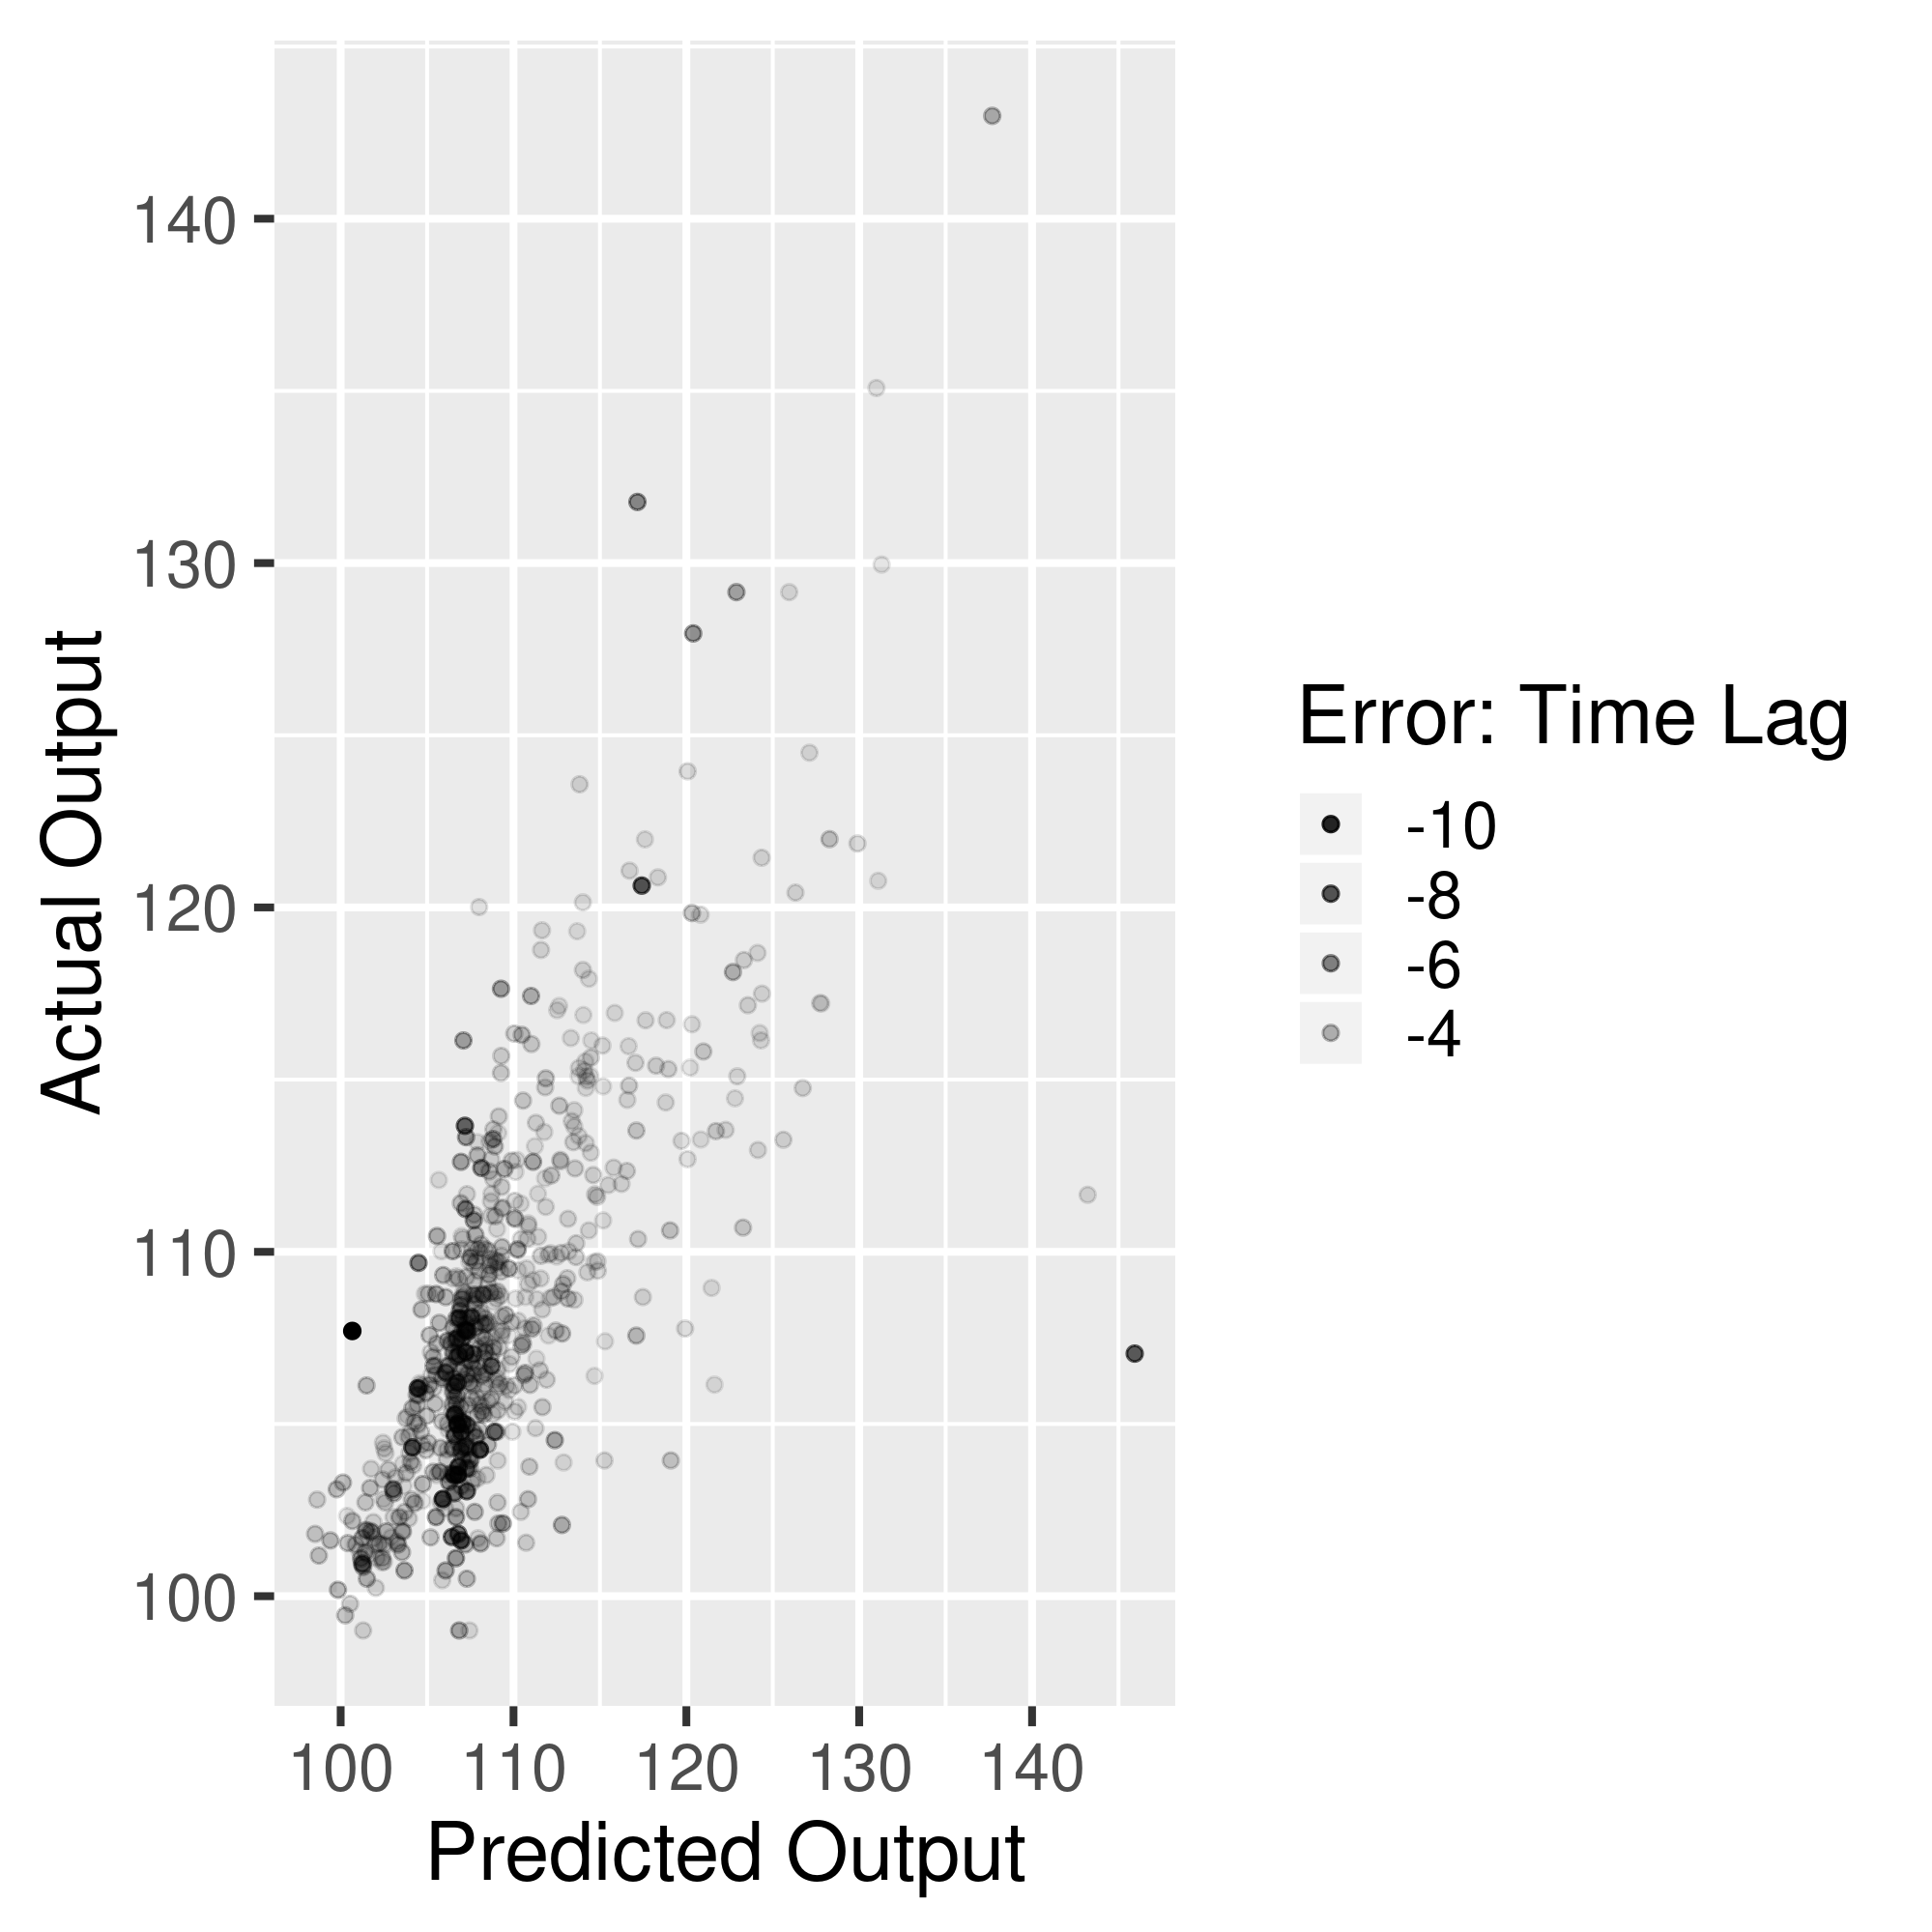
\includegraphics[width=0.5\textwidth]{figures/exp3_lag_error_jus.png}}
\vspace{.3in}
\caption{\textbf{Problem III}, Predicted vs Actual Outputs for the cases with time lag error $\leq -2.5$.}
\label{fig:problem3_lag_error_jus}
\end{figure}



%\begin{table}[h]
%\caption{\textbf{Problem III}: Statistics of the Output distribution} \label{table:problem3_stats}
%\begin{center}
%\begin{tabular}{ll}
%\textbf{Statistic}  &\textbf{Value} \\
%\hline \\
%Minimum         & $111.7$ \\
%$1$st Quartile  & $182.3$ \\
%Median          & $252.1$ \\
%$3$rd Quartile  & $334.5$ \\
%Maximum         & $687.4$ \\
%\end{tabular}
%\end{center}
%\end{table}


\subsubsection{Problem IV}

Figures \ref{fig:problem4_scatter}, \ref{fig:problem4_error}, \ref{fig:problem4_curves} summarize 
the results of the experiment. This case is different as compared to the previous problems as there 
is now a monotonic relationship between the output and time lag. A key difference in the model 
performance in this problem can be observed in error scatter chart \ref{fig:problem4_error}, 
we can see that the time lag errors are symmetric.


\begin{figure}[h]
\vspace{.3in}
\centerline{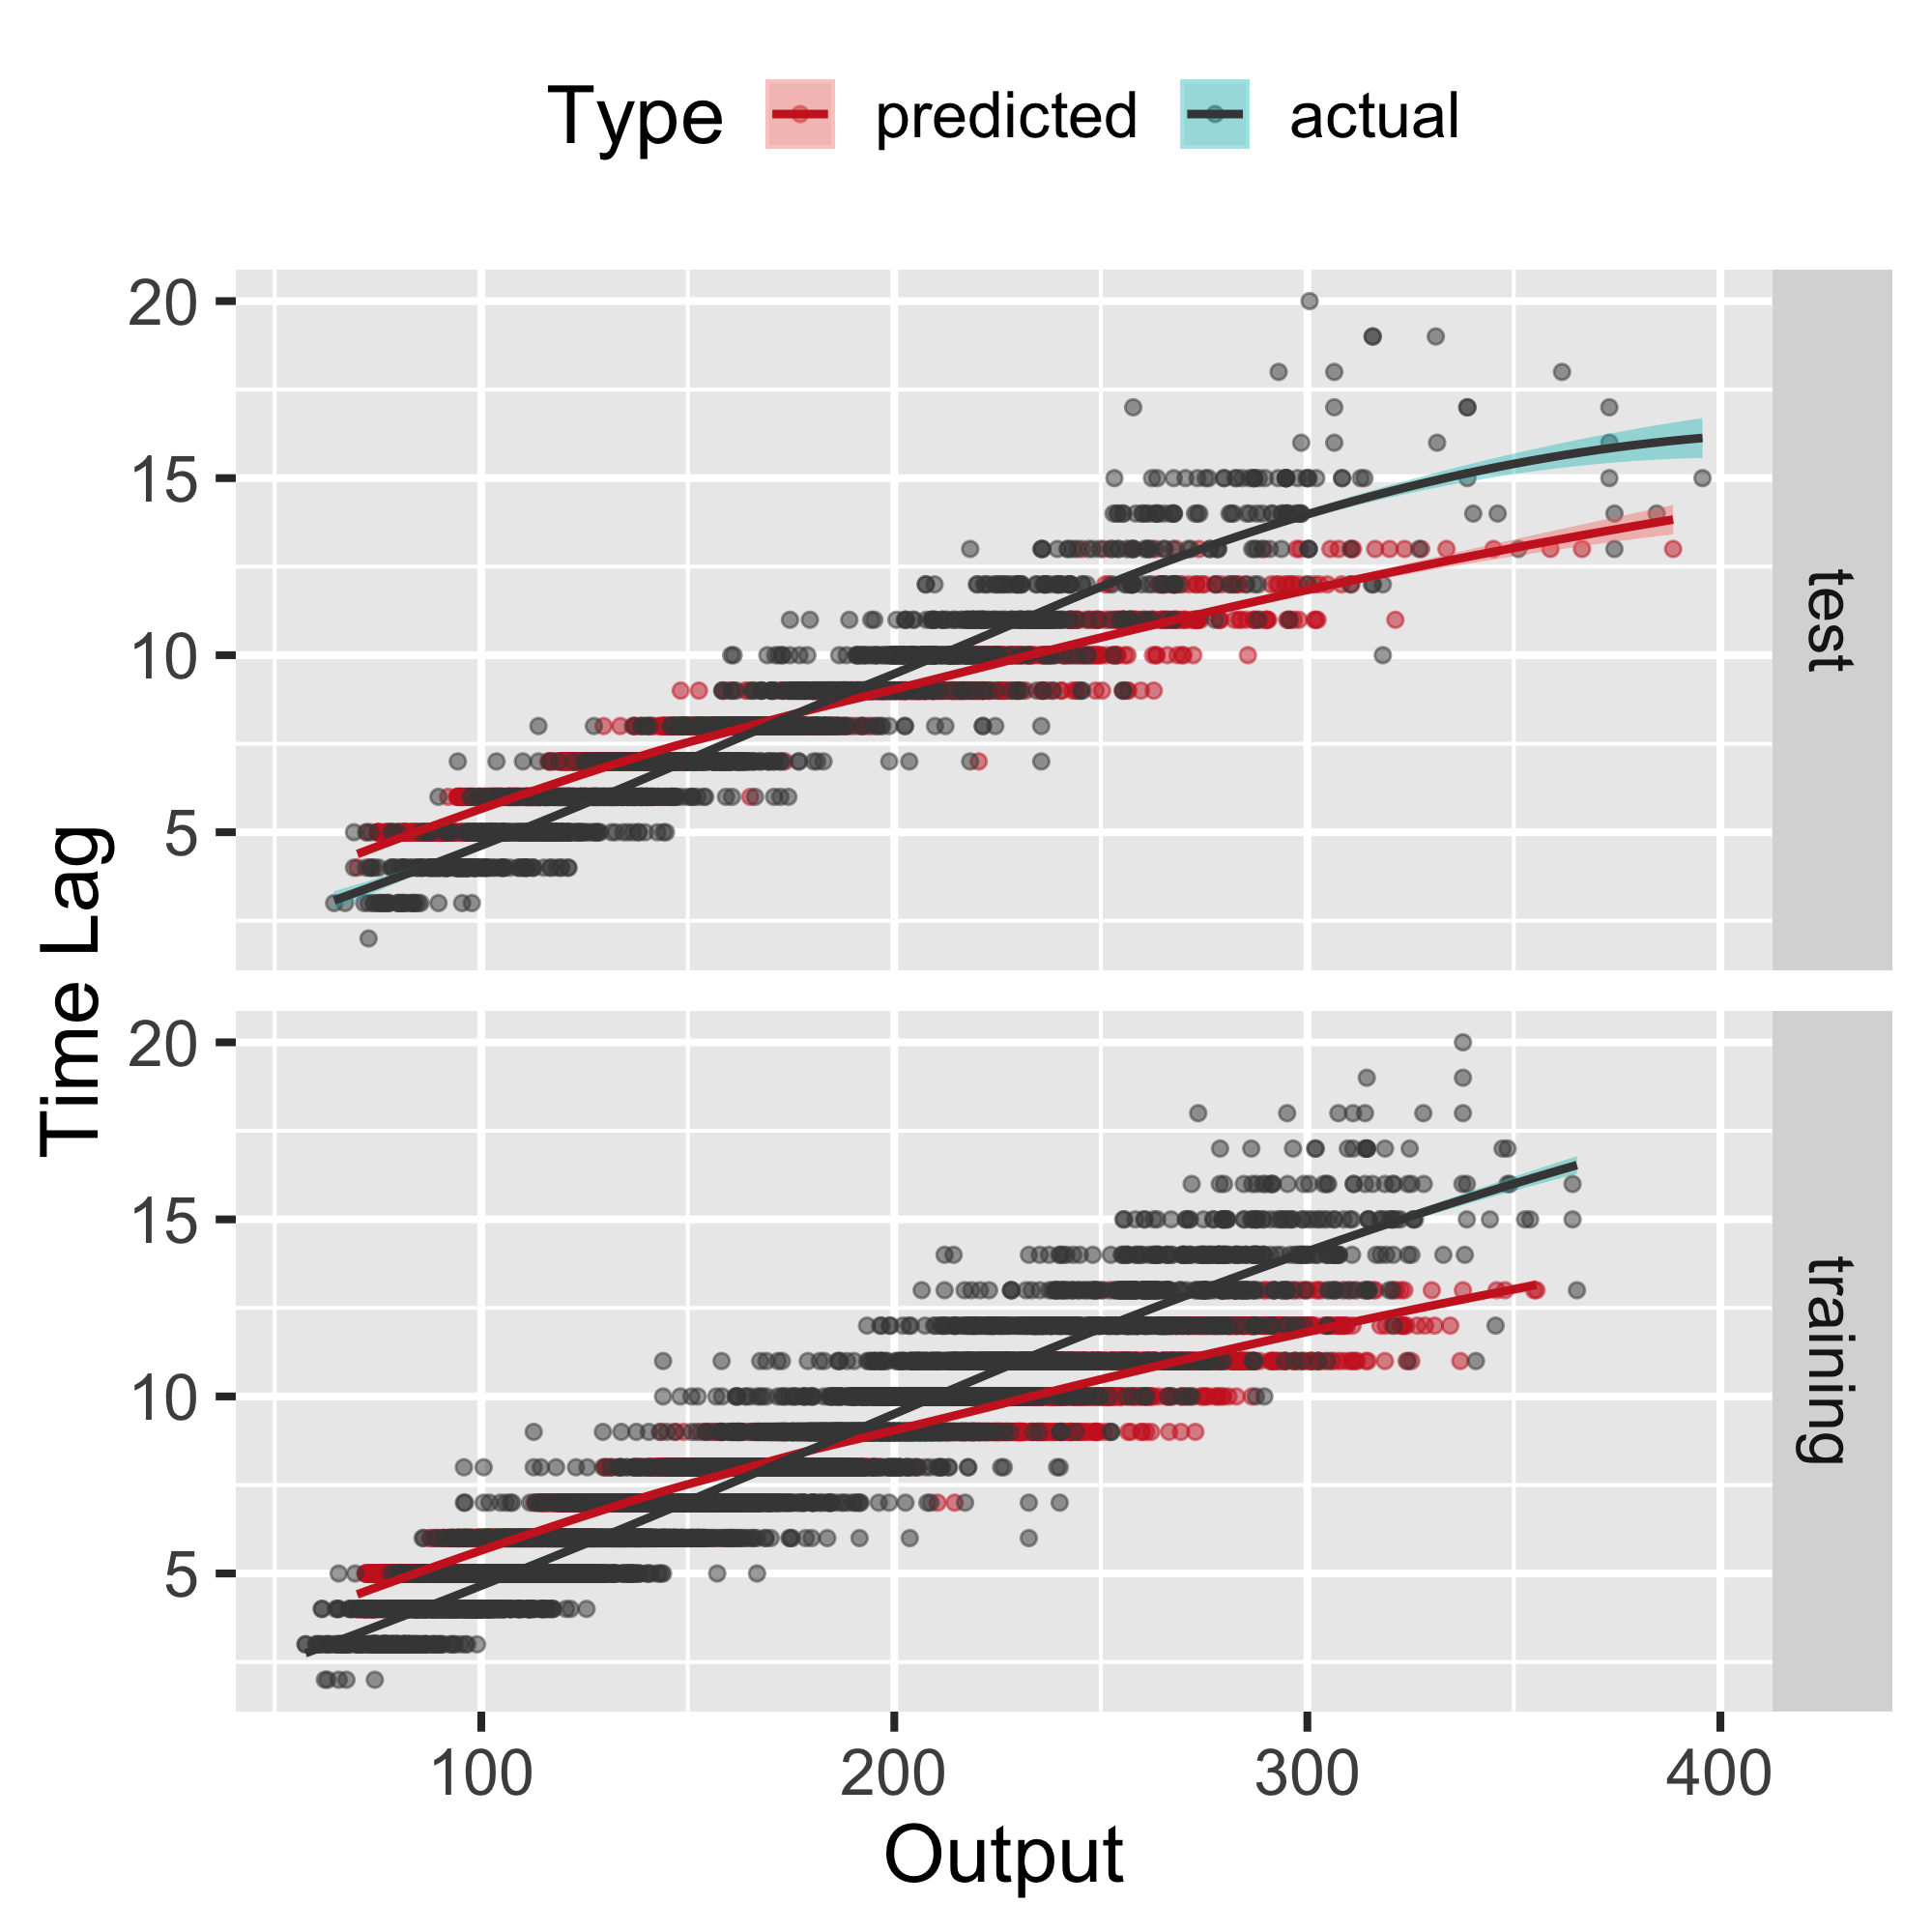
\includegraphics[width=0.5\textwidth]{figures/exp4_scatter_v_tl.png}}
\vspace{.3in}
\caption{\textbf{Problem IV}, Output-Time Lag Scatter plot; model predictions in red and actual data in black}
\label{fig:problem4_scatter}
\end{figure}

\begin{figure}[h]
\vspace{.3in}
\centerline{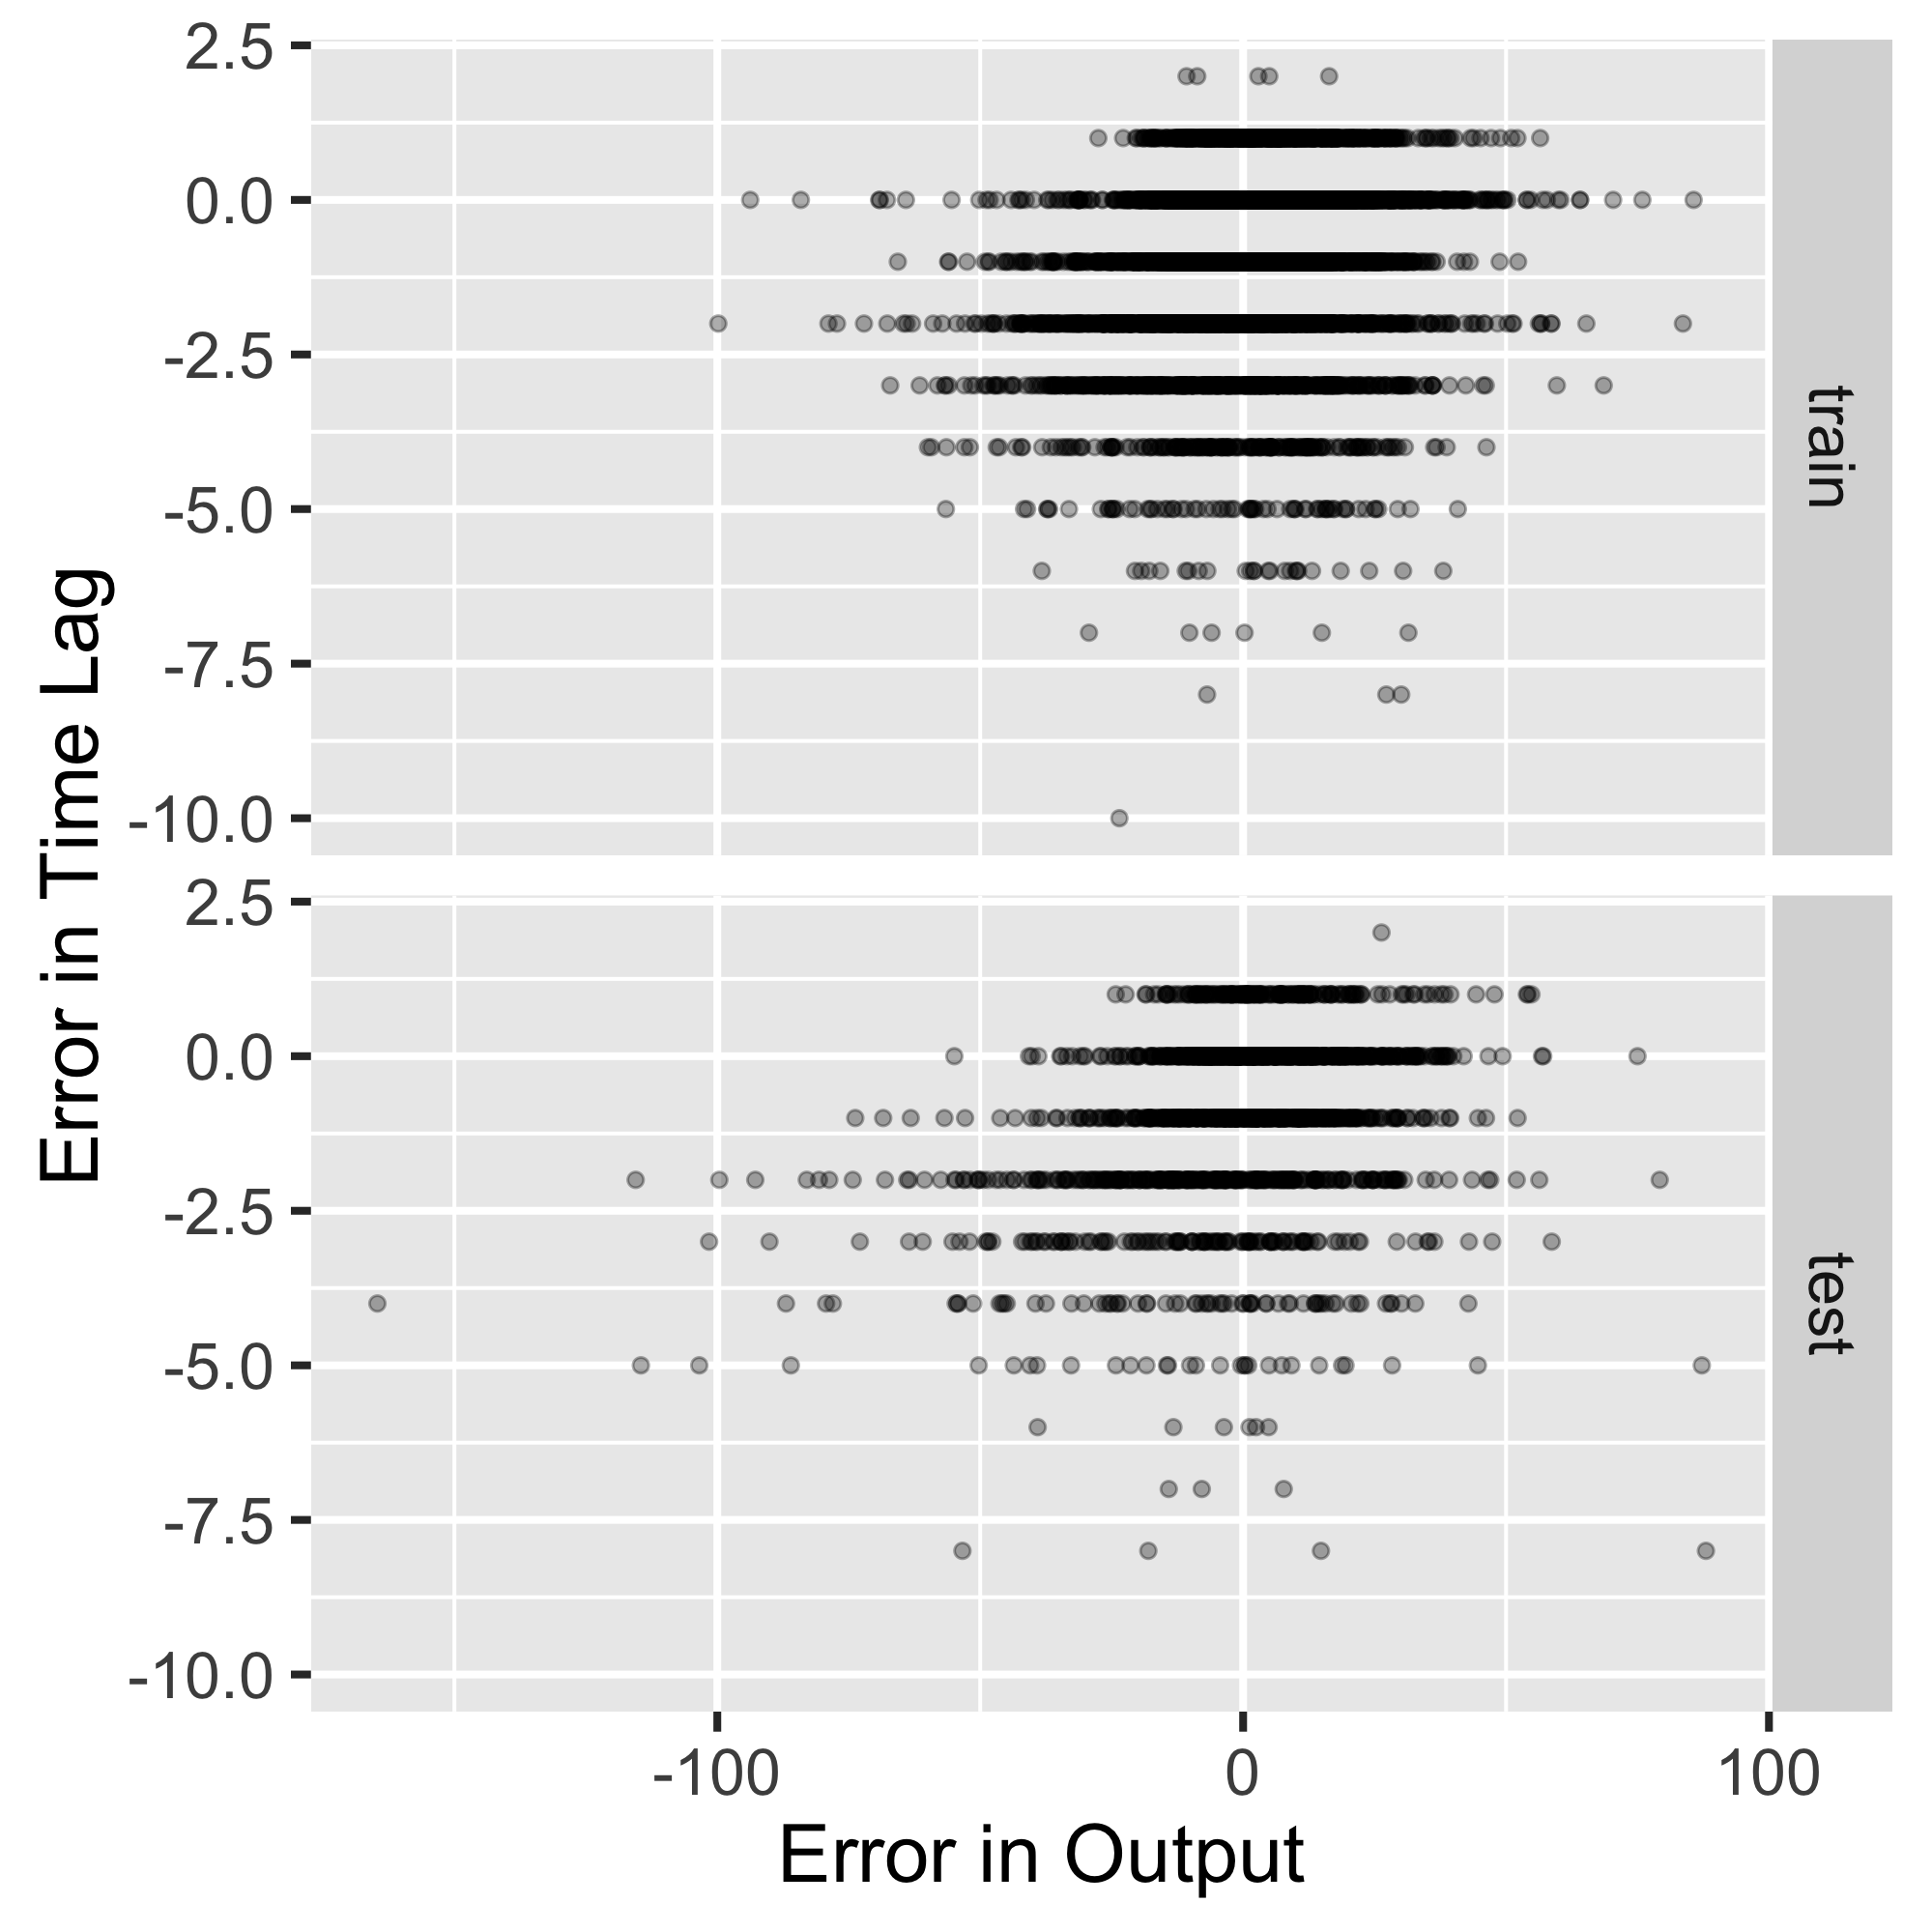
\includegraphics[width=0.5\textwidth]{figures/exp4_scatter_errors.png}}
\vspace{.3in}
\caption{\textbf{Problem IV}, Error in prediction of output vs error in time lag prediction}
\label{fig:problem4_error}
\end{figure}

\begin{figure}[h]
\vspace{.3in}
\centerline{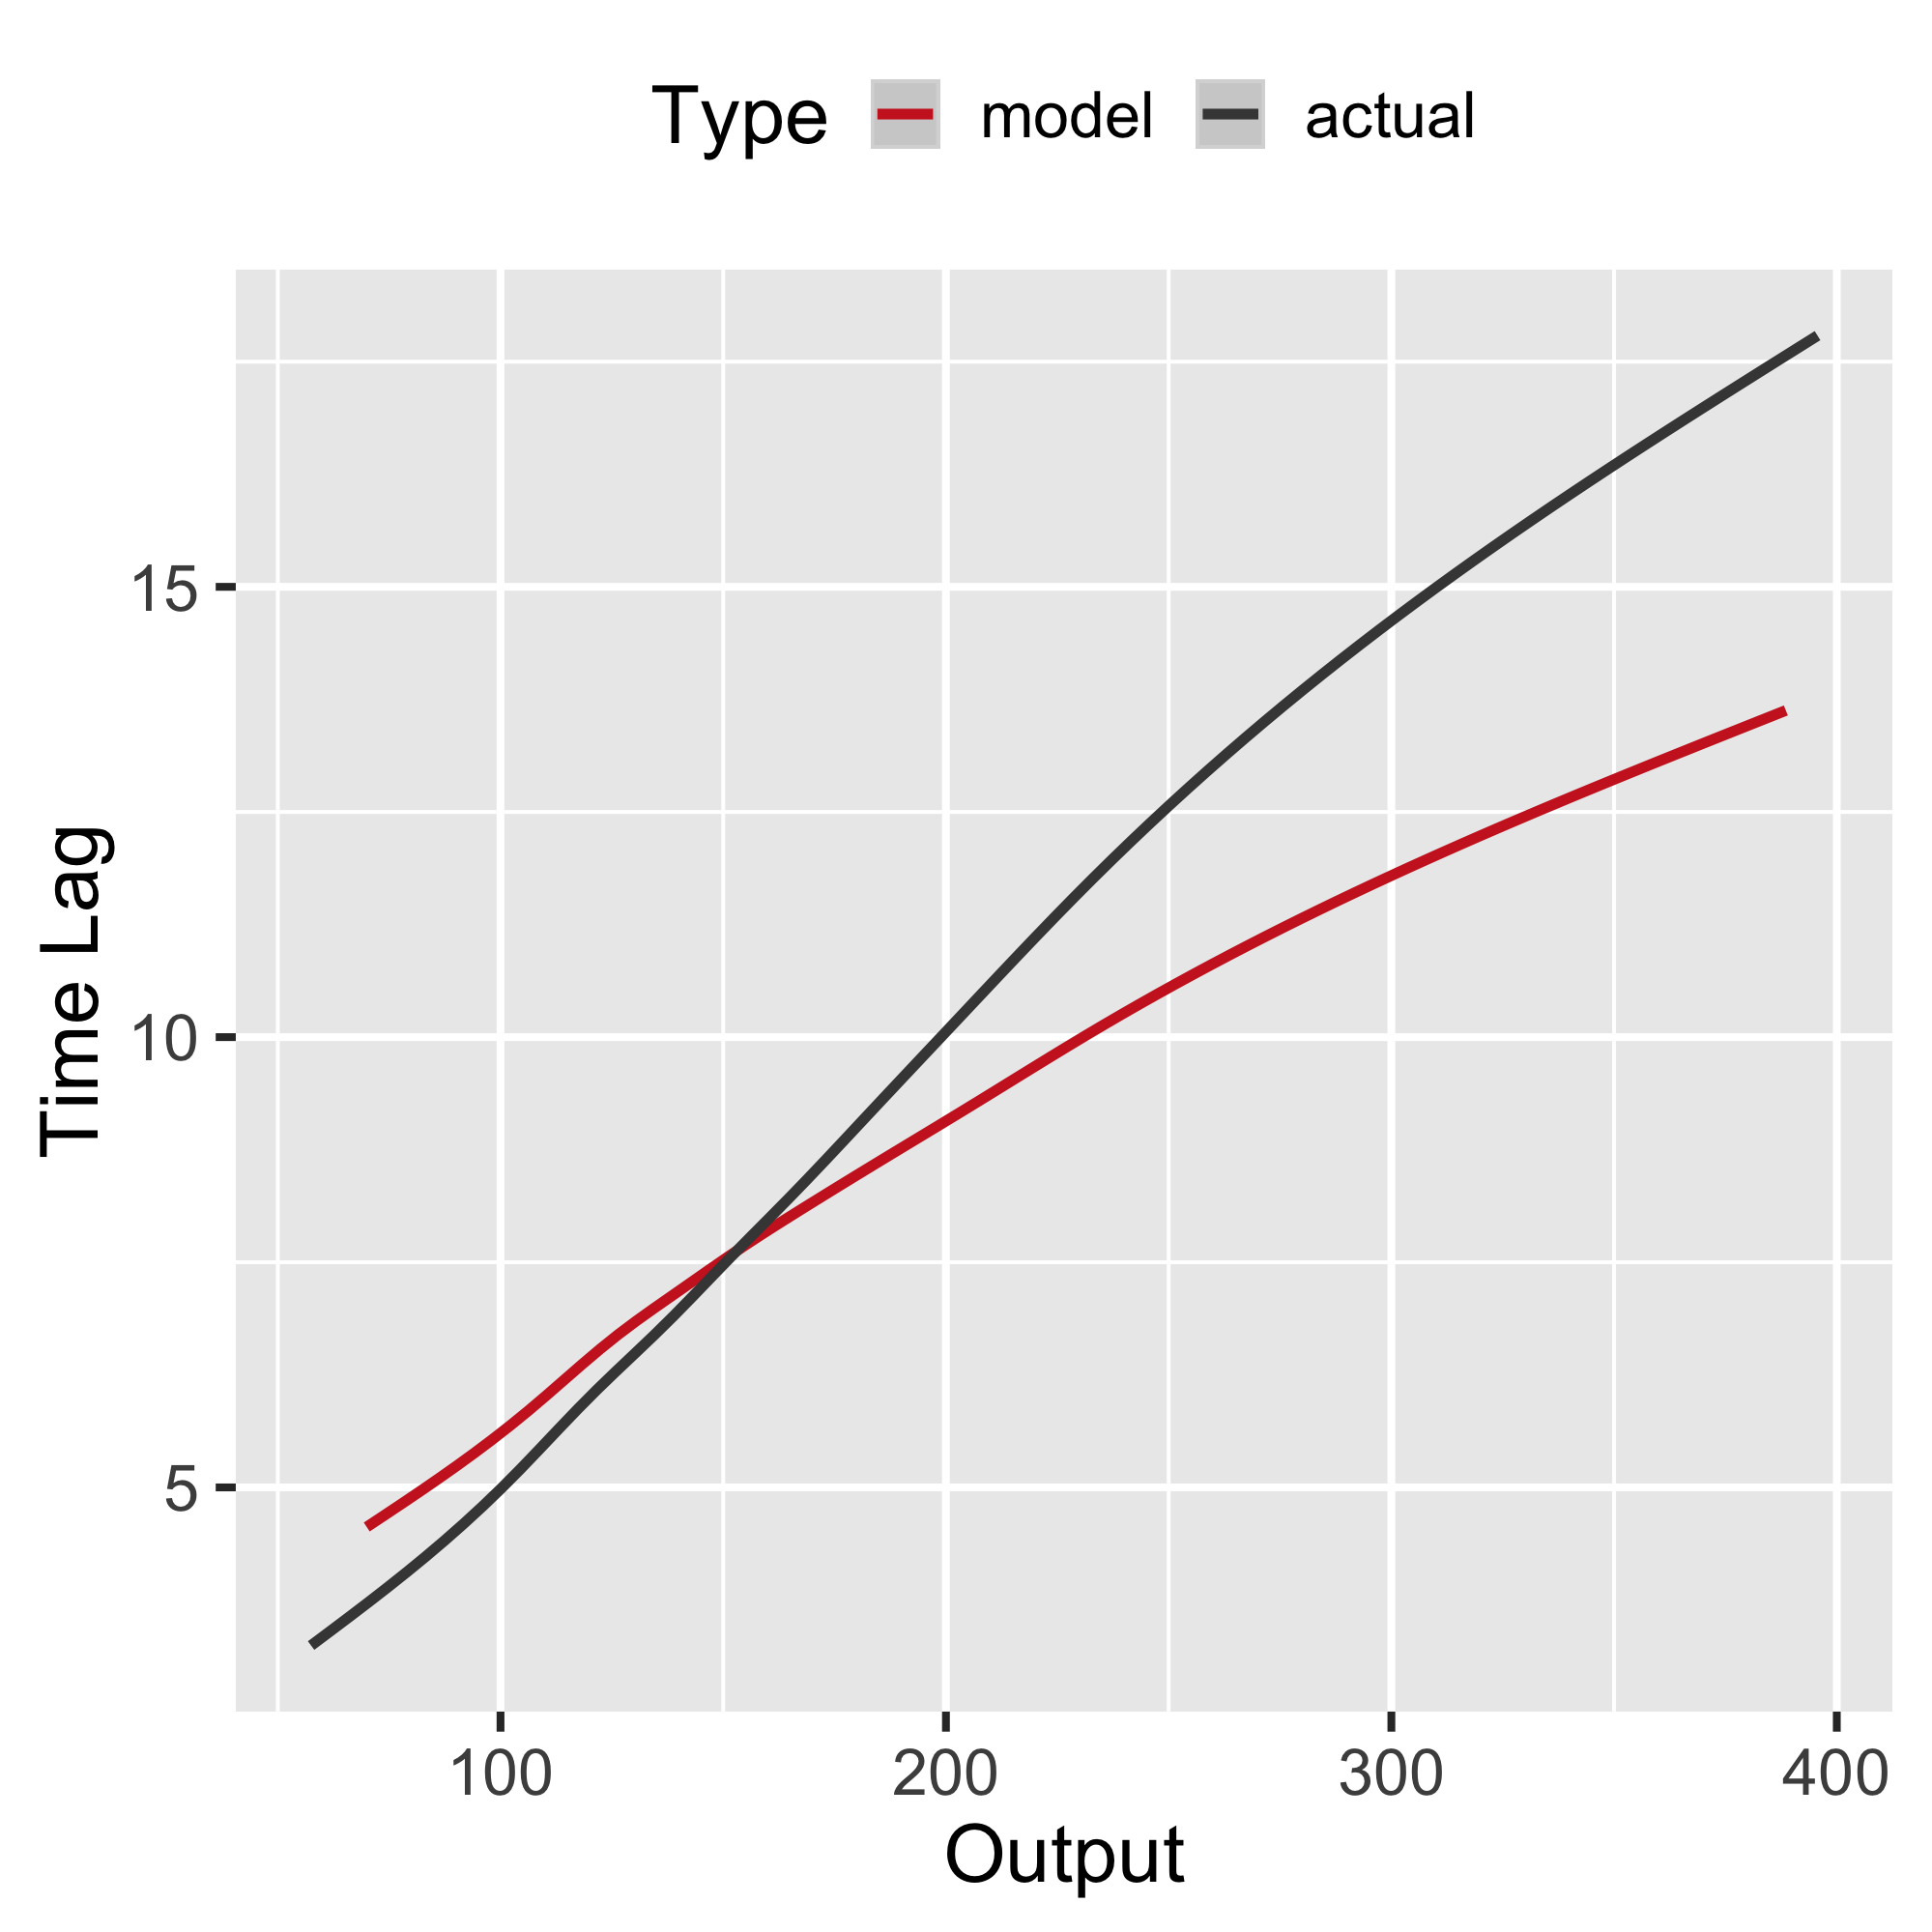
\includegraphics[width=0.5\textwidth]{figures/exp4_predictive_curves.png}}
\vspace{.3in}
\caption{\textbf{Problem IV}, Output vs Time Lag Relationship}
\label{fig:problem4_curves}
\end{figure}

\section{Conclusions}

We present in this work a formulation and a novel solution methodology for the problem of performing 
inference and forecasting in the context of lagged causal relationships between time series. 
We call this problem \emph{Causal Dynamic Time Lag} (CDT) to note the non-stationary nature of the 
causal link between time series $x(t)$ and $y(t)$. We outline a neural network based solution to this 
problem and benchmark its performance on a set of carefully constructed problems.

This work is an area of active research and progress. Going ahead we plan to apply this methodology 
to the problem of forecasting of geomagnetic phenomena which are driven by features observed on the 
surface of the Sun, i.e. sunspots and active regions.


\subsubsection*{Acknowledgements}

\clearpage
\bibliography{references}

\end{document}
